
%%%%%%%%%%%%%%%%%%%%%%%%%%%%%%%%%%%%%%%%%%%%%%%  テンプレート非依存部(開始)  %%%%%%%%%%%%%%%%%%%%%%%%%%%%%%%%%%%%%%%%%%%%%%%  

% \setlength\textfloatsep{18pt}%  between figure and text
% \setlength\abovecaptionskip{4pt}% between figure and caption
% \setlength\floatsep{18pt}% between figures

\comment{TBD:1-1, 1-14, 2-2, 3-5}

% \IEEEraisesectionheading{\chapter{Introduction}\label{sec:introduction}}
\chapter{Introduction}
\label{chap:introduction}
\comment{1-4, 1-5, 1-6, 2-1, 2-4}
The evolution of a next-generation computing platform oriented toward having multi-/many-core platforms is necessary to satisfy the demand for increasing computation in conjunction with reasonable power consumption in several domains such as automobiles.
This trend is also adapted to embedded systems because of high processing requirements.
For example, self-driving systems involve various applications and are sometimes characterized by demands for high-performance computing.
Considering the requirements of high processing, predictability, and energy efficiency for self-driving systems, such systems require a heterogeneous computing system such as multi-/many-core platforms and graphical processing units (GPU).
(This is discussed in Chapter \ref{chap:related_work}.)
\comment{1-3} In embedded systems, multi-/many-core architectures are an important trend as the architecture integrates cores to realize high-performance and general-purpose computing with low power consumption \cite{becker2016contention}, \cite{perret2016mapping}.
Extant studies have examined several applications of multi/many-core platforms \cite{becker2016contention}, \cite{saidi2015shift}, \cite{perret2016temporal}, \cite{perret2016mapping}, \cite{becker2014mapping}, \cite{BURGIO2017299}.
% Recently, the computational ability of single core processors has reached its limit \comment{1-3} and thus the applicability of Moore's law \cite{moore2006cramming} is unclear.
% Multi/many core architecture is an important trend in \comment{1-3} recent years as it integrates cores to realize high-performance and general-purpose computing with low power consumption.
% Hence, high energy efficiency is a superior feature of multi/many core platforms.

% As detailed in the preceding paragraph, the demand for increasing computation in conjunction with reasonable power consumption drives the need for multi/many core architecture in several domains.
% Real-time embedded systems are an example in which multi/many core platforms are adopted since they face increasing processing requirements.
% Extant studies have examined numerous applications of multi/many cores platforms \cite{becker2016contention}, \cite{saidi2015shift}, \cite{perret2016temporal}, \cite{perret2016mapping}, \cite{becker2014mapping}.

% For example, automotive systems involve various applications and are sometimes characterized by demands for high-performance computing.
% Automotive applications are responsible for several control systems such as the powertrain, chassis, steering wheel, driver assistance and user interface.
% Advanced driver assistance systems are characterized by increasing complexity and computational requirements and necessitate intelligence such as an self-driving driving system.
% Moreover, they also require significant energy efficiency and cost reduction.
% Although modern automotive systems are composed of several Electronic Control Unit (ECU) managing subsystems, there is a shift from numerous scattered ECUs to hierarchical multi/many core Domain Controllers (DC).
% Evidently, a hybrid scenario is also applicable. 
% \comment{1-4}
% Specifically, DCs combine performance with low power consumption to realize high parallel processing and power efficiency.
% \comment{1-5}
% % Furthermore, flexible scalability of a many-core platform facilitates development efficiency.

% A related example involves avionics systems that also include various applications and require cost efficiency.
% \comment{1-6}
% % Multi/many core platforms can be applied in the avionics domain due to their highly integrated characteristics and increasing processing demands.
% Low power consumption of cores leads to lower cooling requirements, and this is a critical issue for avionics.
% Multi/many core platforms reduce energy consumption as well as the costs and weight.
% Weight reduction is the most important factor for avionics, and integration with a multi/many core platform reduces the number of processing boards and cooling units.
% Thus, an integrated platform results in space, weight and cost reductions.

Based on the above background, multi/many-core platforms are fabricated and released as commercial off-the-shelf (COTS) multicore components.
(e.g., the Massively Parallel Processor Arrays (MPPA) 256 developed by Kalray \cite{de2014time}, Tile-Gx developed by Tilera \cite{ramey2011tile} \cite{schooler2010tile}, Tile-64 developed by Tilera \cite{bell2008tile64}, Xeon Phi developed by Intel \cite{chrysos2014intel}, \cite{chrysos2012intel}, and Single-chip Cloud Computer (SCC) developed by Intel \cite{baron2010single})
Several platforms such as MPPA-256 and Tile-64 target embedded systems, and the research focused on multi-/many-core platforms has received increasing attention \cite{kanter2015kalray}, \cite{denet2017work}, \cite{perret2016predictable}.
We discuss comparisons of many-core platforms in Chapter \ref{chap:related_work}.

In embedded many-core platforms, nonuniform memory access (NUMA) and distributed memories connected with network-on-chip (NoC) components are an important approach for core scalability and power consumption.
Several COTS platforms include NoC technology and a cluster of many-core architectures in which cores are \comment{1-7} allocated closely.
For instance, MPPA-256 and Tile-Gx72 have NoC components to share distributed memories instead of shared buses.
Furthermore, MPPA-256 contains 16 clusters in which 16 cores are included and contains 256 general-purpose cores in total.
Although the cores do not guarantee cache coherency, this significantly exceeds the number of cores in other COTS such as Tile-64 and Tile-Gx72.
The clusters of cores are capable of running separate independent applications with respect to the desired power envelope of embedded applications.

Despite the appearance of embedded many-core platforms, several difficulties persist in the adaptation of these platforms in embedded domain \cite{becker2016contention}, \cite{saidi2015shift}.
In NoC-based embedded many-core platforms, researches on NoC-based many-core platforms do not fully reveal data transfer between distributed memories with NoC technology, memory access characteristics in NUMA, and parallelization potential in practical applications for application developers.
Additionally, reuse of existing software application is difficult because application developers have to write platform oriented codes for NoC data transfer between clusters.
For example, writing software for robotics system including self-driving system is difficult, particularly as the scale and scope of embedded software application continues to grow.

To meet these challenges, we conduct evaluations to reveal the practicality of NoC-based many-core platforms and propose software framework called ROS-lite similar to Robot Operating System (ROS) \cite{quigley2009ros}, \cite{rosorg} for reuse of existing applications and efficient development on heterogeneous computing platforms.
ROS, an open-source robot operating system, is structured communications layer above the host operating systems of a heterogeneous compute cluster and has been being rapidly developed and widely used in the robotics community \cite{cousins2011exponential}.
(Please refer to Apendix A: Robot Operating System (ROS).)
This work explores scalable parallel computing and data allocation with quantitative evaluations and a practical application.
As a reference embedded many-core platform, we have implemented evaluation program, practical applications, and ROS-lite on MPPA-256 \cite{de2014time} which adopts NUMA using NoC technology and realizes numerous cores with low power consumption.
% The timing requirement of real-time embedded systems continues to warrant solutions.
% The impact of integrating applications in multi/many-core platforms is not completely understood to date.
% This is a critical issue because embedded systems have requirements for reliable and predictable behavior.

% Considering embedded requirements, multi/many cores need NUMA because of scalability of the number of cores and reasonable power consumption.
% Scalable data allocation enhances parallelized high-performance and general-purpose computing with low power consumption.
% MPPA-256 is one of the commercial off-the-shelf (COTS) multi/many-core components targeting embedded system and adopts distributed memory architecture with NoC. (We discusses comparison to other platforms in Section \ref{sec:related_work}.)
% However, its data transfer between distributed memories with NoC, parallelization potential, and memory access characteristics are not fully unrvealed for application developers.
% This work explores above issues with quantitative evaluations and a practical application.

\textbf{Contributions:}
\comment{1-1, 3-3: To be clarified}
This work focuses on examining embedded many-core computing based on NoC technology, such as MPPA-256.
We conduct evaluations of data transfer methods on NoC components and microbenchmarks with matrix calculation to clarify latency characteristics of data transfer, parallel computing, and the influence of data allocation.
Subsequently, we parallelize a localization algorithm that is the core of the self-driving system.
Finally, this paper for the first time presents a light weight ROS architecture supporting NoC called ROS-lite on embedded many-core platforms.
We reveal the advantages and disadvantages of embedded many-core computing based on NoC technology in a quantitative manner by introducing the following contributions:

\begin{itemize}
  \setlength{\leftskip}{-5mm}
  \item On DMA-capable NoC components, the evaluations of the data transfer quantitatively characterize the end-to-end latencies, which depend on the routing and DMA configurations, and the memory access speed, which varies according to where data are allocated and what accesses the memory.
  \item In many-core platforms based on NoC technology, the scalability of parallelization is observed in evaluations of matrix calculations in several situations and a real complex application as a part of a self-driving system.
  \item Under limited memory, our proposed software framework provides structured communications layer and efficient development on heterogeneous computing platforms including NoC.
\end{itemize}

To the best of our knowledge, this is the first work that examines data transfer and data allocation matters for many-core computing beyond an intuitive expectation to allow system designers to choose appropriate data transfer methods.
Additionally, the speed-up result of a self-driving application indicates a practical potential for NoC-based embedded many-core computing.
\comment{1-8, 1-9}
% It is expected that the findings of this study will potentially be applicable to several types of many-core architectures as opposed to just MPPA-256.
% Therefore, the contributions of this study can be used in low-latency many-core computing.

\textbf{Organization:}
\memo{Add ROS-lite section}
The remainder of this work is organized as follows.
The system model considered in this work is discussed in Chapter \ref{chap:system_model} in which the hardware model, namely Kalray MPPA-256 Bostan, and the system model are presented.
\comment{1-10}
Chapter \ref{chap:evaluations} explains evaluation setup and approach, and illustrates experimental evaluations.
Chapter \ref{chap:related_work} examines the related work that focuses on multi-/many-core systems.
Chapter \ref{chap:conclusion} presents the conclusions and directions for future research.


\chapter{System Model}
\label{chap:system_model}
This section presents the system model used throughout the work.
The many-core model of Kalray MPPA-256 Bostan is considered.
First, a hardware model is introduced in Section \ref{sec:hardware_model}, followed by a software model in Section \ref{sec:software_model}.

\section{Hardware Model}
\label{sec:hardware_model}
The MPPA-256 processor is based on an array of computing clusters (CCs) and I/O subsystems (IOSs) that are connected to NoC nodes with a toroidal two-dimensional topology 
(as shown in Figs. \ref{fig:mppa_architecture}, \ref{fig:cc_architecture} and \ref{fig:noc_map}).
The MPPA many-core chip integrates 16 CCs and 4 IOSs on NoC.
The architecture of Kalray MPPA-256 is presented in this section.

\subsection{I/O Subsystems (IOS)}
\label{sec:ios}
MPPA-256 contains the following four IOSs: North, South, East, and West.
The North and South IOSs are connected to a DDR interface and an eight-lane PCIe controller.
The East and West IOSs are connected to a quad 10 Gb/s Ethernet controller.
Two pairs of IOSs organize two I/O clusters (IOCs), as shown in Fig. \ref{fig:mppa_architecture}.
Each IOS consists of quad IO cores and a NoC interface.

\begin{itemize}
  \setlength{\leftskip}{-5mm}    
  \item \textbf{IO Cores}: IO cores are connected to a 16-bank parallel shared memory with a total capacity (IO SMEM) of 2 MB, as shown in Fig. \ref{fig:mppa_architecture}.
  The four IO cores have their own instruction cache 8-way associative corresponding to 32 ($8 \times 4$) KB and share a data cache 8-way with 128 KB and external DDR access.
  The sharing of the data cache of 128 KB allows coherency between the IO cores.
  Additionally, IO cores operate controllers for PCIe, Ethernet, \comment{1-11}and other I/O devices.
  They operate the local peripherals, including NoC interfaces with DMA.
  It is also possible to conduct an application run on the IO cores.
  
  \item \textbf{NoC Interface}: The NoC interface contains four DMA engines (DMA1-4) and four NoC routers, as shown in Fig. \ref{fig:mppa_architecture}, and the IOS DMA engine manages transfers between the IO SMEM, IOS DDR, and IOS peripherals (e.g., PCIe interface and Ethernet controllers).
  The DMA engine transfers data between routers via NoC through NoC routers and has the following three NoC interfaces: a receive (Rx) interface, a transmit (Tx) interface, and a microcore (UC).
  The UC is a fine-grained multithreaded engine that can be programmed to set threads sending data with a Tx interface.
  The UC can extract data from memory by using a programmed pattern and send the data on the NoC.
  After the UC is initiated, this continues in an autonomous fashion without using a processing element (PE) and an IO core.
\end{itemize}
\begin{figure*}[!htbp]
  \centering
  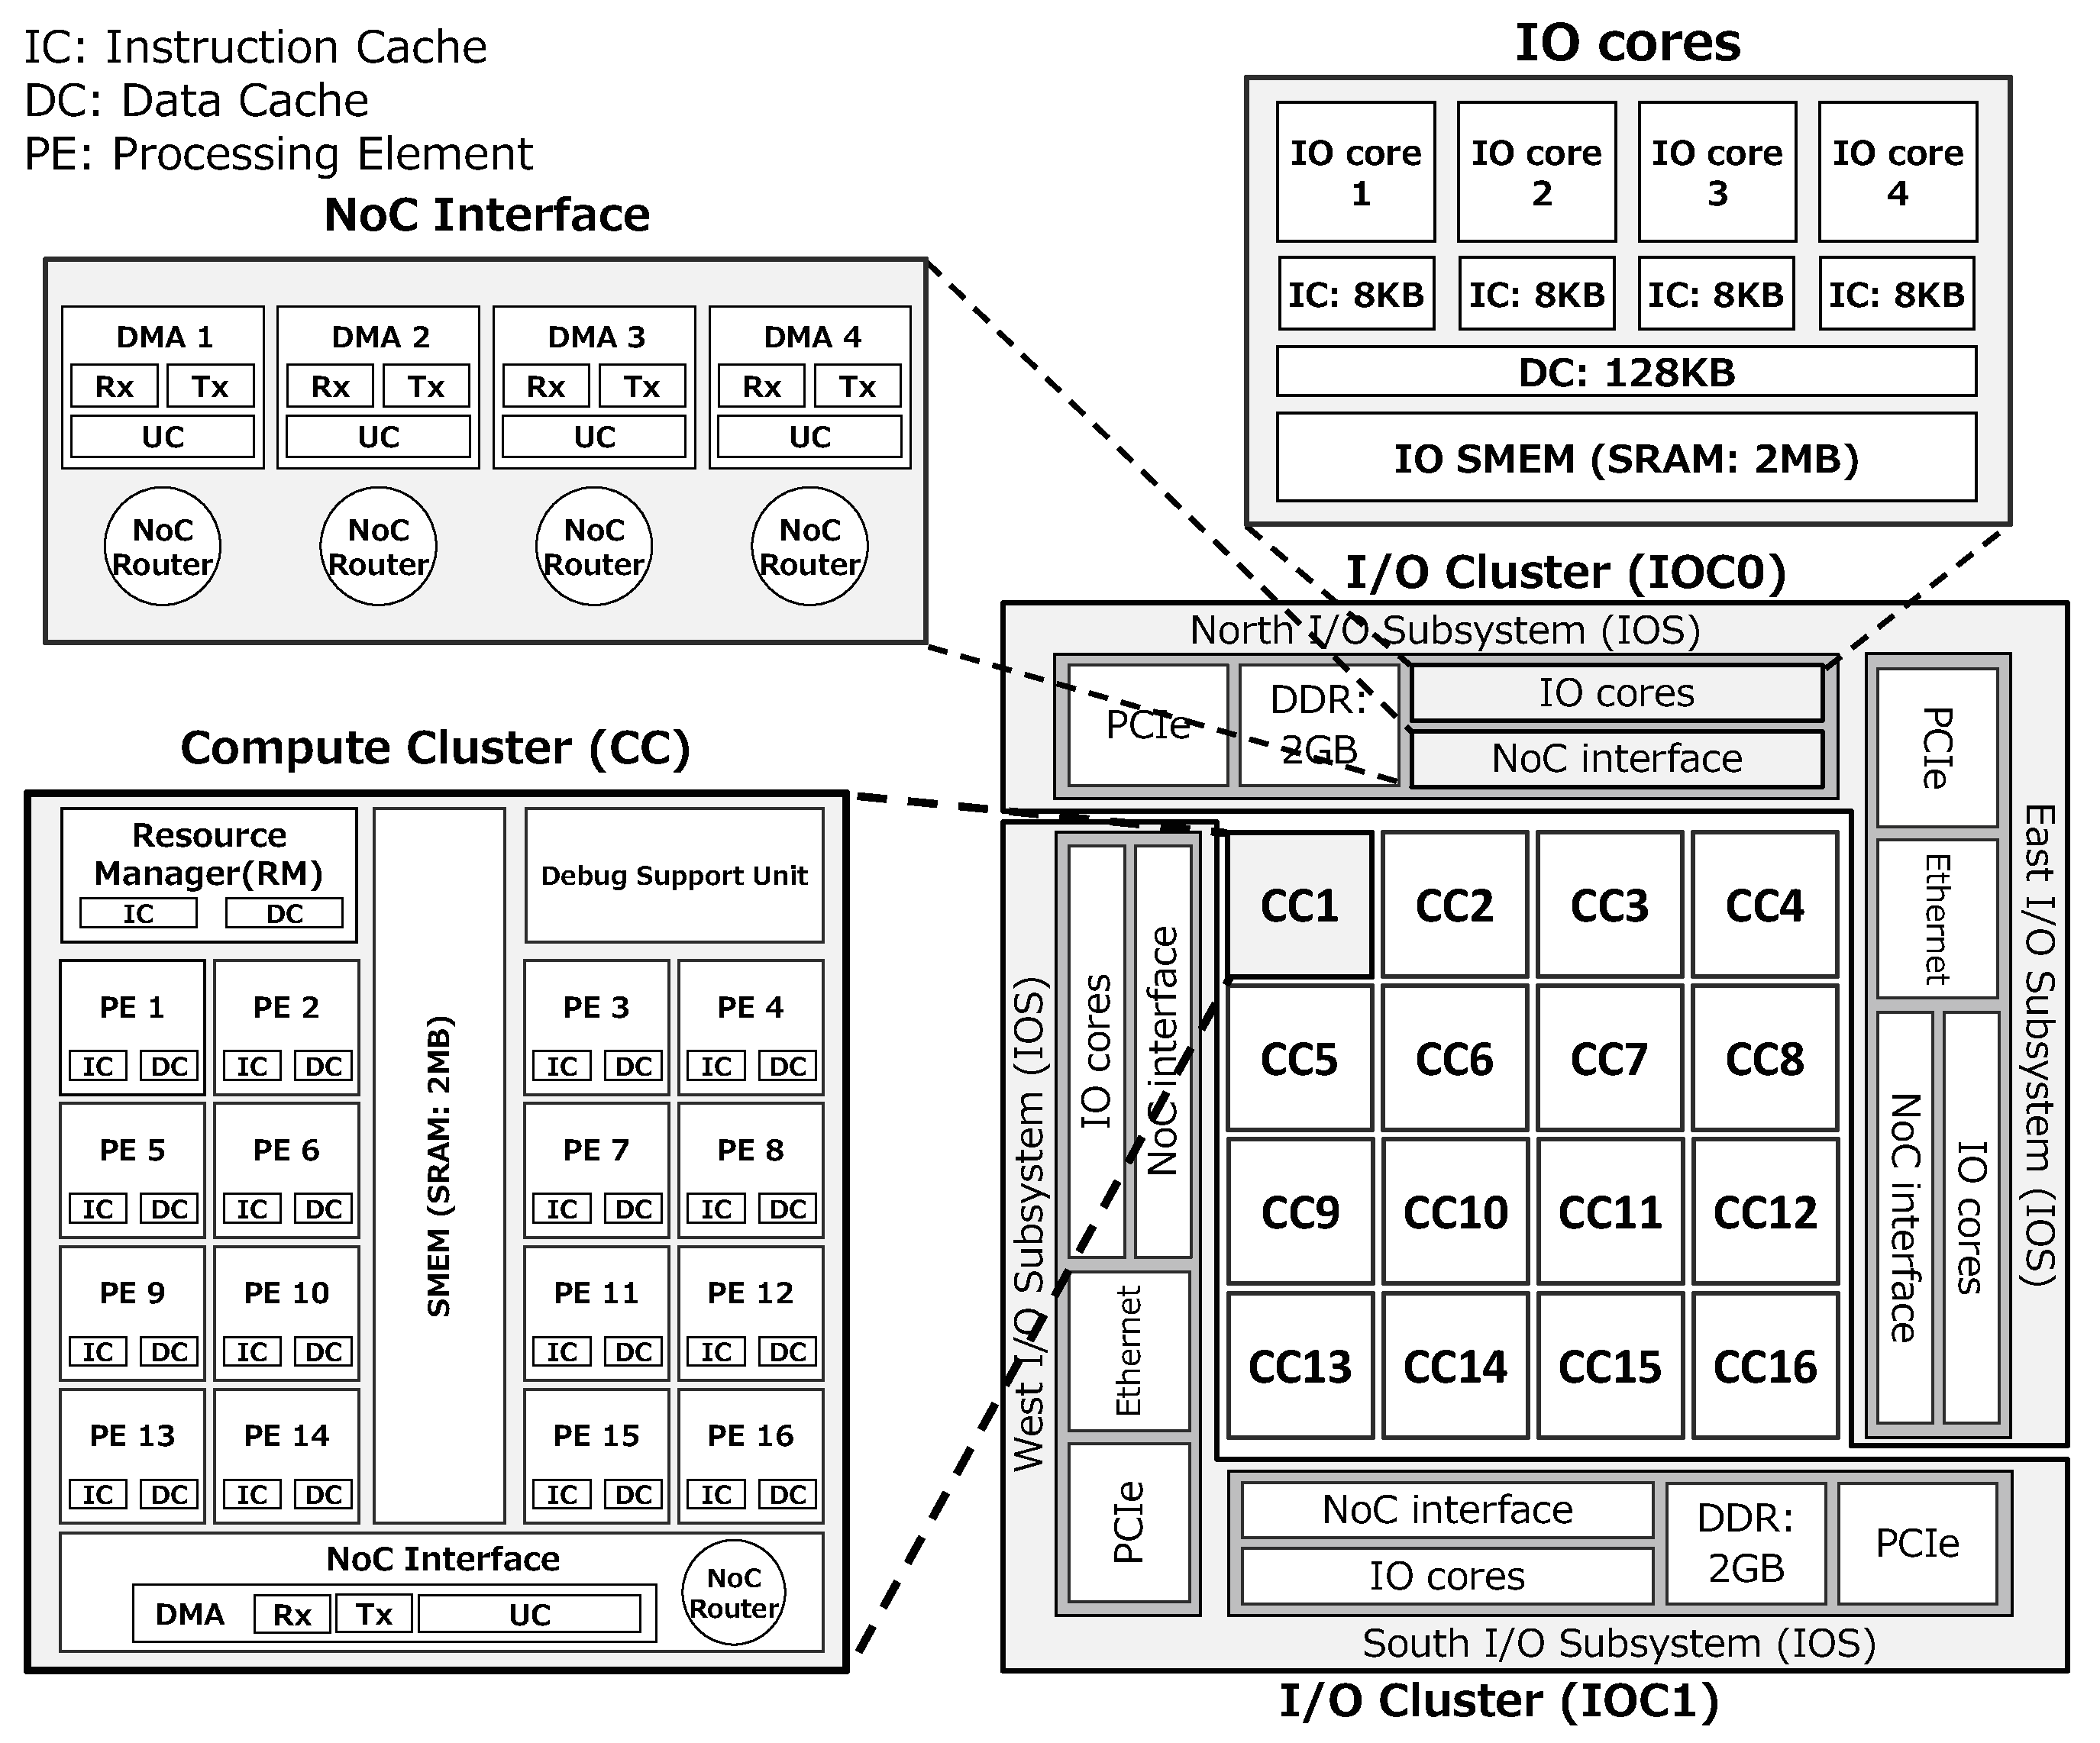
\includegraphics[width=0.9\linewidth]{../figure/mppa_architecture.eps}
      \caption{\label{fig:mppa_architecture}
    An overview of the architecture of the Kalray MPPA-256 Bostan.}
  \end{figure*}

\subsection{Compute Clusters (CCs)}
\label{sec:cc}
In MPPA-256, the 16 inner nodes of the NoC correspond to the CCs.
Fig. \ref{fig:cc_architecture} illustrates the architecture of each CC.

\begin{itemize}
  \setlength{\leftskip}{-5mm}    
  \item \textbf{PEs and an RM}:
  \comment{2-3}
  In a CC, 16 PEs and an RM share 2 MB cluster local memory (SMEM), so that 17 k1-cores (a PE or the RM) share 2 MB SMEM.
  % The capacity of each SMEM bank is 128 KB.
  Users use the PEs primarily for parallel processing.
  Developers spawn computing threads on PEs.
  The PEs and an RM in the CC correspond to the Kalray-1 cores, which implement a 32-bit 5-issue Very Long Instruction Word architecture with 600 or 800 MHz.
  Each core is fitted with its own instruction and data caches.
  Each cache is 2-way associative with a capacity of 8 KB.
  Note that these caches do not guarantee cache coherency.
  
  \item \textbf{A Debug Support Unit and a NoC Interface}:
  In addition to PEs and an RM, bus masters on the SMEM correspond to a Debug Support Unit and a DMA engine in a NoC interface.
  A DMA engine and a NoC router are laid out in a NoC interface.
  The CC DMA engine also has the following three interfaces: an Rx, a Tx, and a UC. 
  The CC DMA engine is instantiated in every cluster and connected to the SMEM.
\end{itemize}
\begin{figure*}[!htbp]
  \centering
  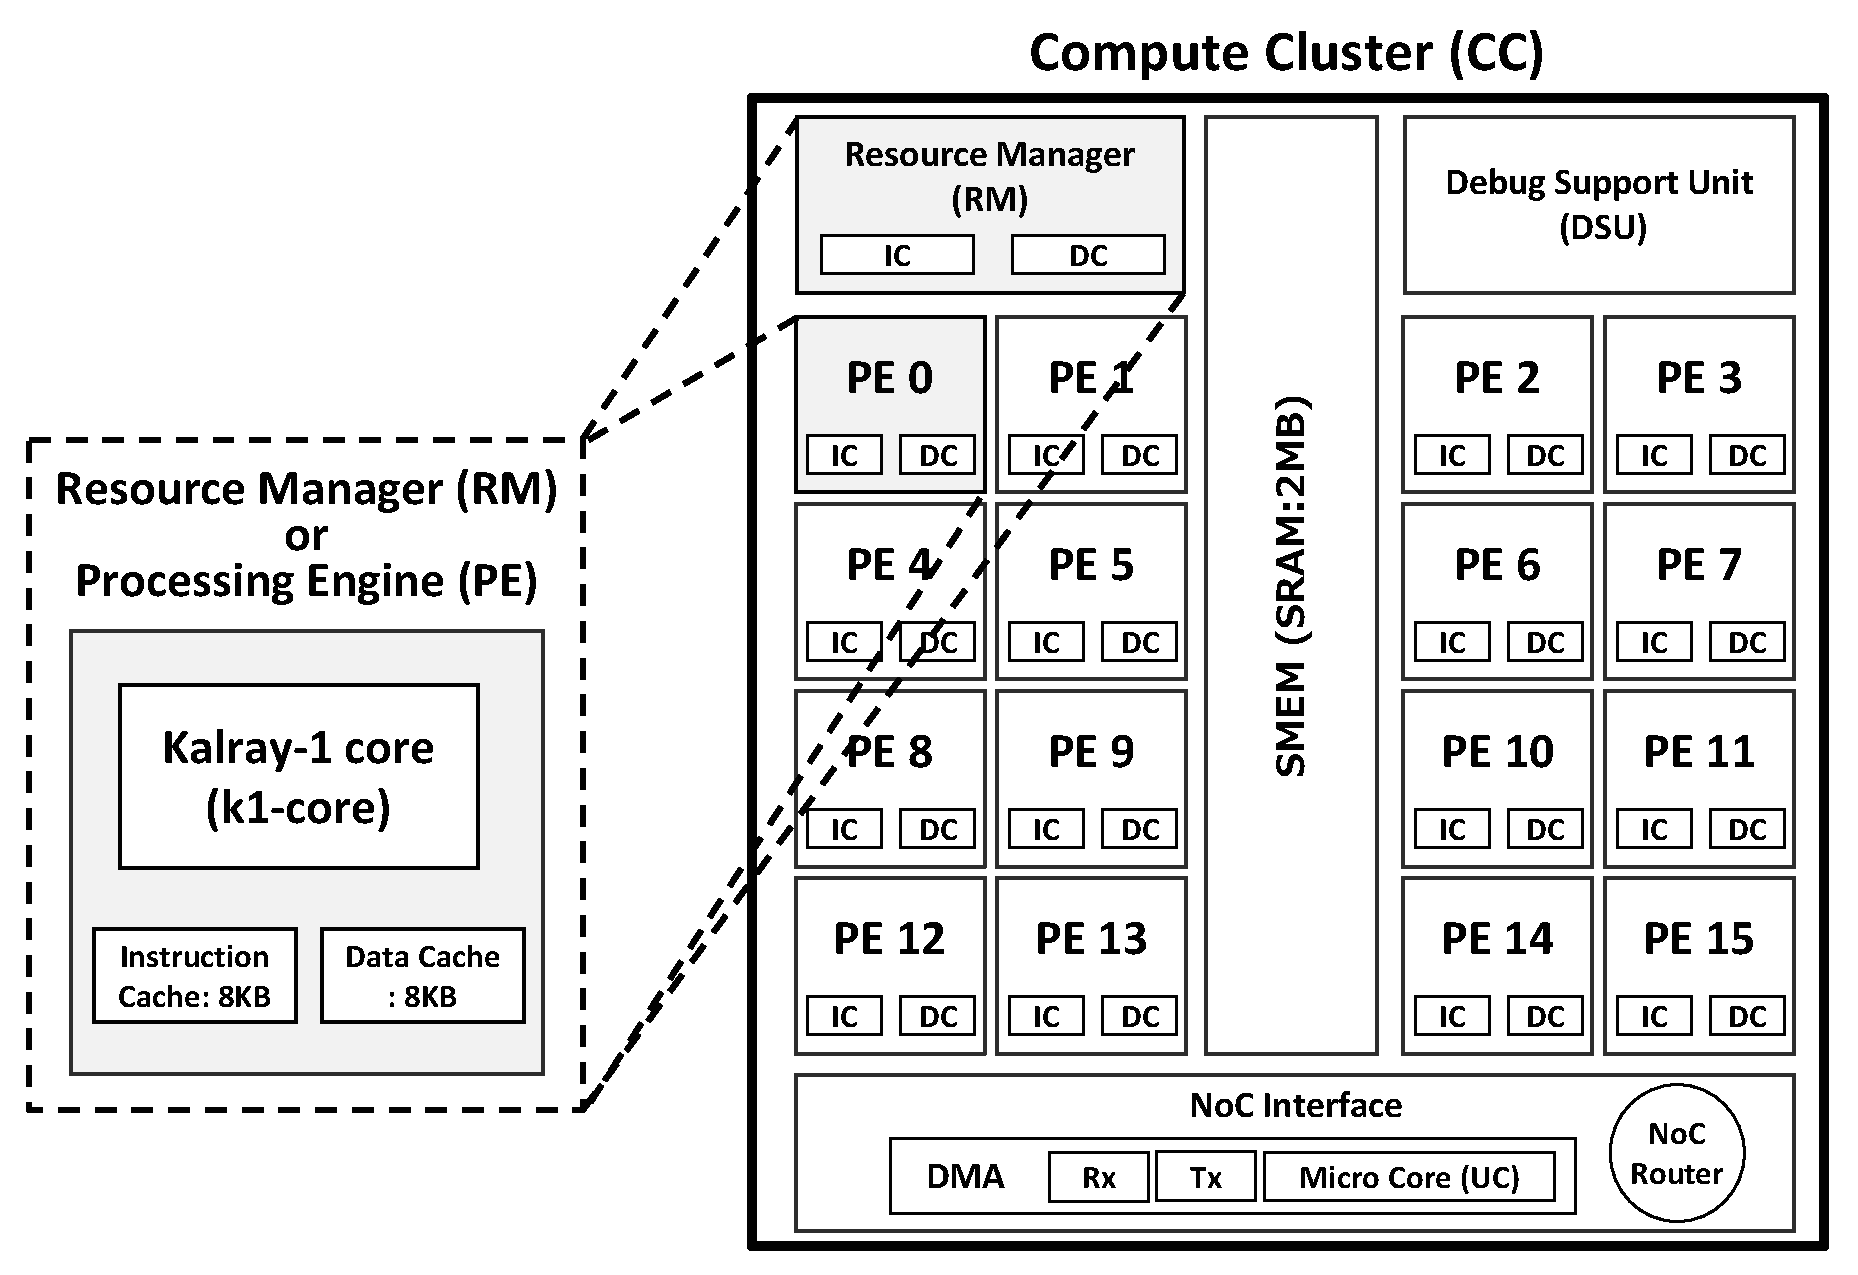
\includegraphics[width=0.7\linewidth]{../figure/cc_architecture.eps}
  \caption{\label{fig:cc_architecture}
    Compute Cluster architecture.}
\end{figure*}

\subsection{Network-on-Chip (NoC)}
\label{sec:noc}
The 16 CCs and the four IOSs are connected by NoC as shown in Fig. \ref{fig:noc_map}.
Furthermore, NoC is constructed \comment{1-12} as the bus network and has routers on each node.

\begin{itemize}
  \setlength{\leftskip}{-5mm}
  \item \textbf{Bus Network}:
  A bus network connects nodes (CCs and IOSs) with torus topology \cite{dally2001route}, which \comment{1-13} involves a low average number of hops when compared to mesh topology \cite{vangal200780}, \cite{taylor2002raw}.
  The network is actually composed of the following two parallel NoCs with bidirectional links (denoted by red lines in Fig. \ref{fig:noc_map}):
  the data NoC (D-NoC) that is optimized for bulk data transfers and the control NoC (C-NoC) that is optimized for small messages at low latency.
  The NoC is implemented with wormhole switching and source routing.
  Data is packaged in variable length packets that are broken into small pieces called flits (flow control digits).
  The NoC traffic is segmented into packets, with each packet including 1-4 header flits and 0-62 payload data flits.
  
  \item \textbf{NoC routers}:
  One node per CC and four nodes per I/O subsystem hold the following two routers of their own: a D-NoC router and a C-NoC router.
  Each RM or IO core on a NoC node is associated with the two aforementioned  NoC routers.
  Furthermore, DMA engines in a NoC interface on the CC/IOS send and receive flits through the D-NoC routers with the Rx interface, the Tx interface, and the UC.
  A mailbox component corresponds to the virtual interface for the C-NoC and enables one-to-one, N-to-one, or one-to-N low-latency synchronization.
  The NoC routers shown in Fig. \ref{fig:cc_architecture} illustrate nodes as R1-16, R128-131, R160-163, R224-227, and R192-195 in Fig. \ref{fig:noc_map}.
  % The NoC routers are illustrated as nodes in Fig. \ref{fig:noc_map}.
  For purposes of simplicity, D-NoC/C-NoC routers are illustrated with a NoC router.
  In both D-NoC and C-NoC, each network node (a CC or an IOS)  includes the following 5-link NoC routers:
  four duplexed links for North/East/West and South neighbors and a duplexed link for local address space attached to the NoC router.
  The NoC routers include FIFOs queuing flits for each direction.
  The data links are four bytes wide in each direction and operate at the CPU clock rates of 600 MHz or 800 MHz, with the result that each tile can transmit/receive a total of 2.4 GB/s or 3.2 GB/s, which is spread across the four directions (i.e., North, South, East, and West).
\end{itemize}  

\clearpage
\begin{figure*}[!htbp]
  \centering
  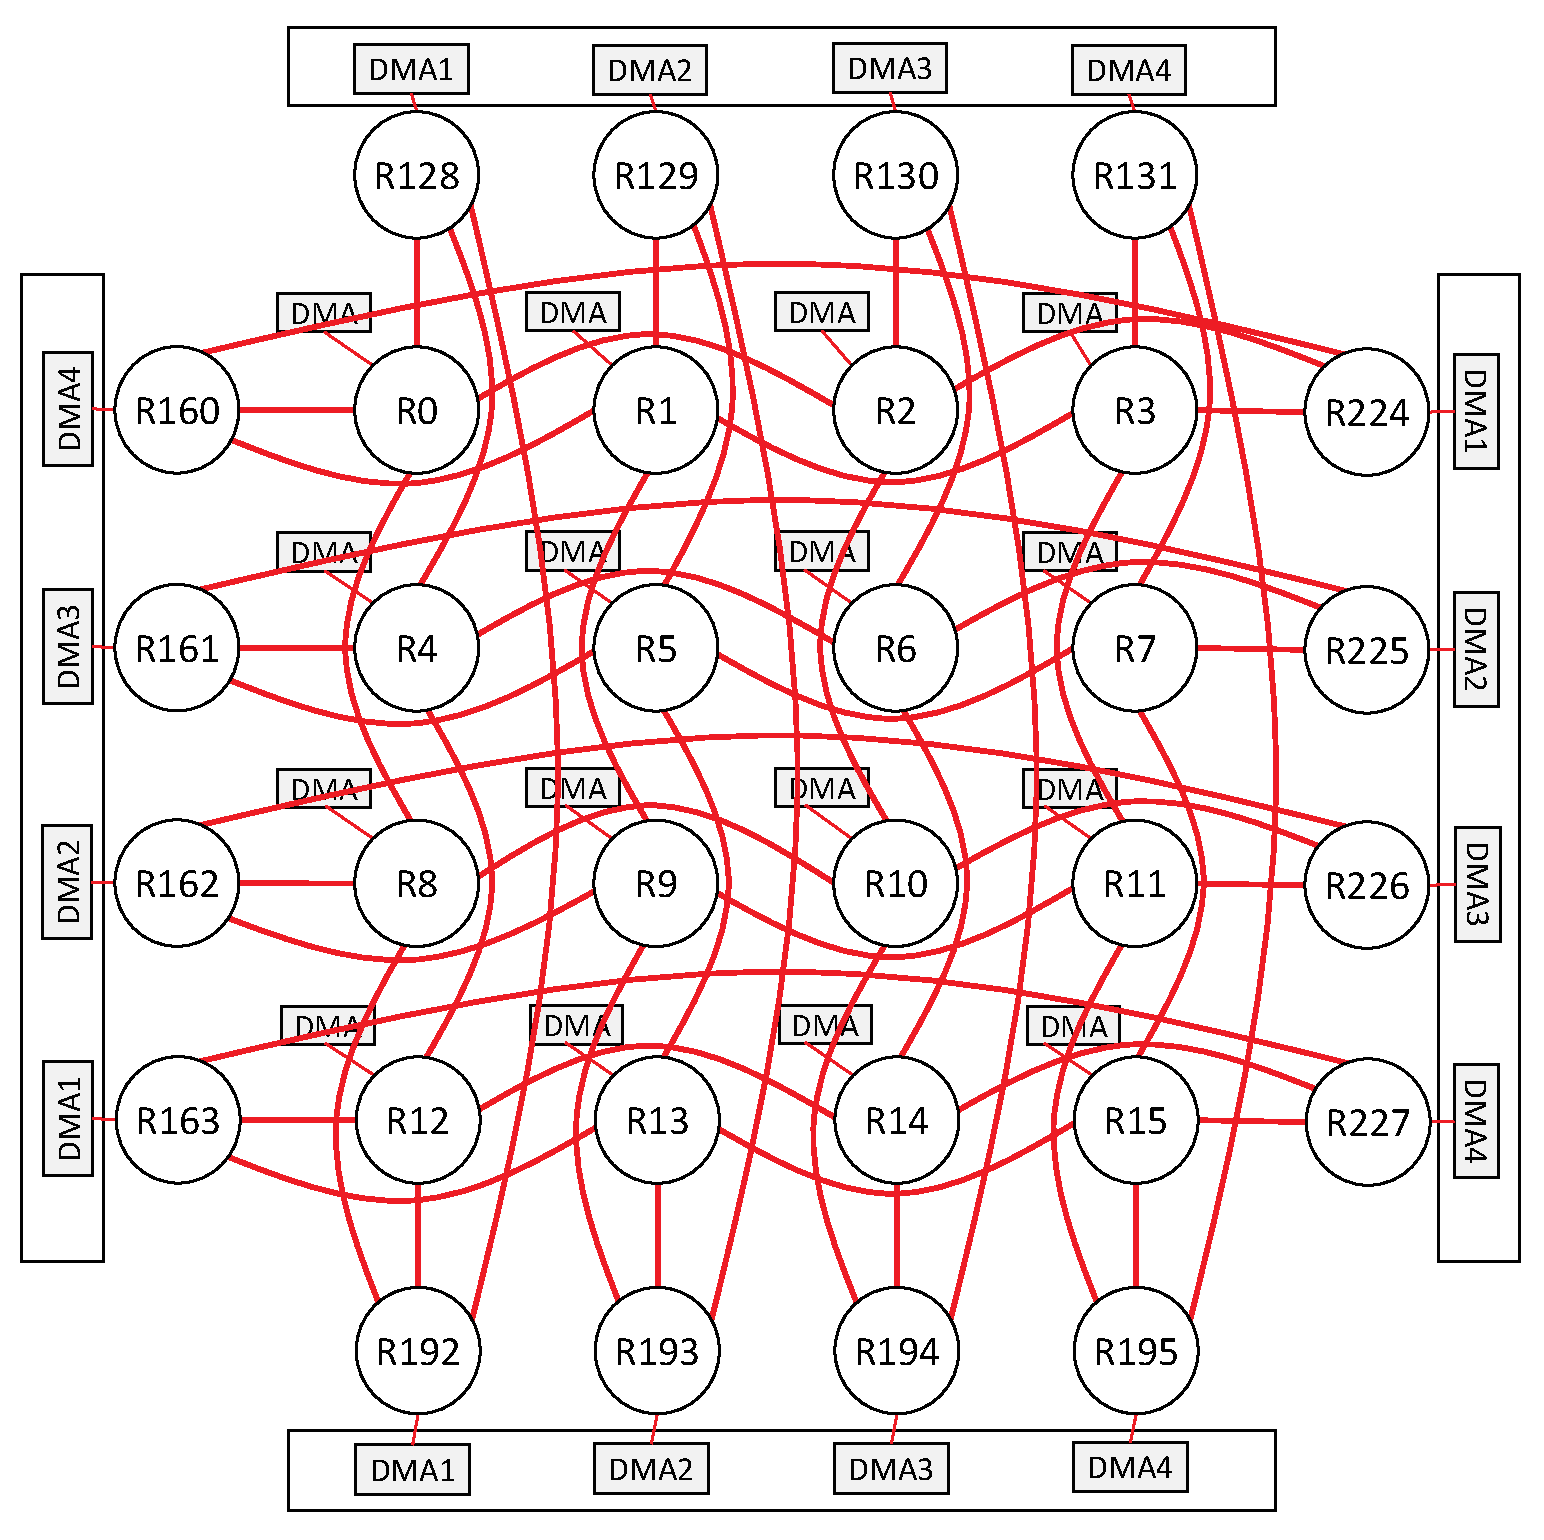
\includegraphics[width=0.7\linewidth]{../figure/noc_map.eps}
      \caption{\label{fig:noc_map}
    NoC connections (both D-NoC and C-NoC).}
\end{figure*}
\clearpage

\section{Software Model}
\label{sec:software_model}

\begin{figure*}[!htbp]
  \centering
  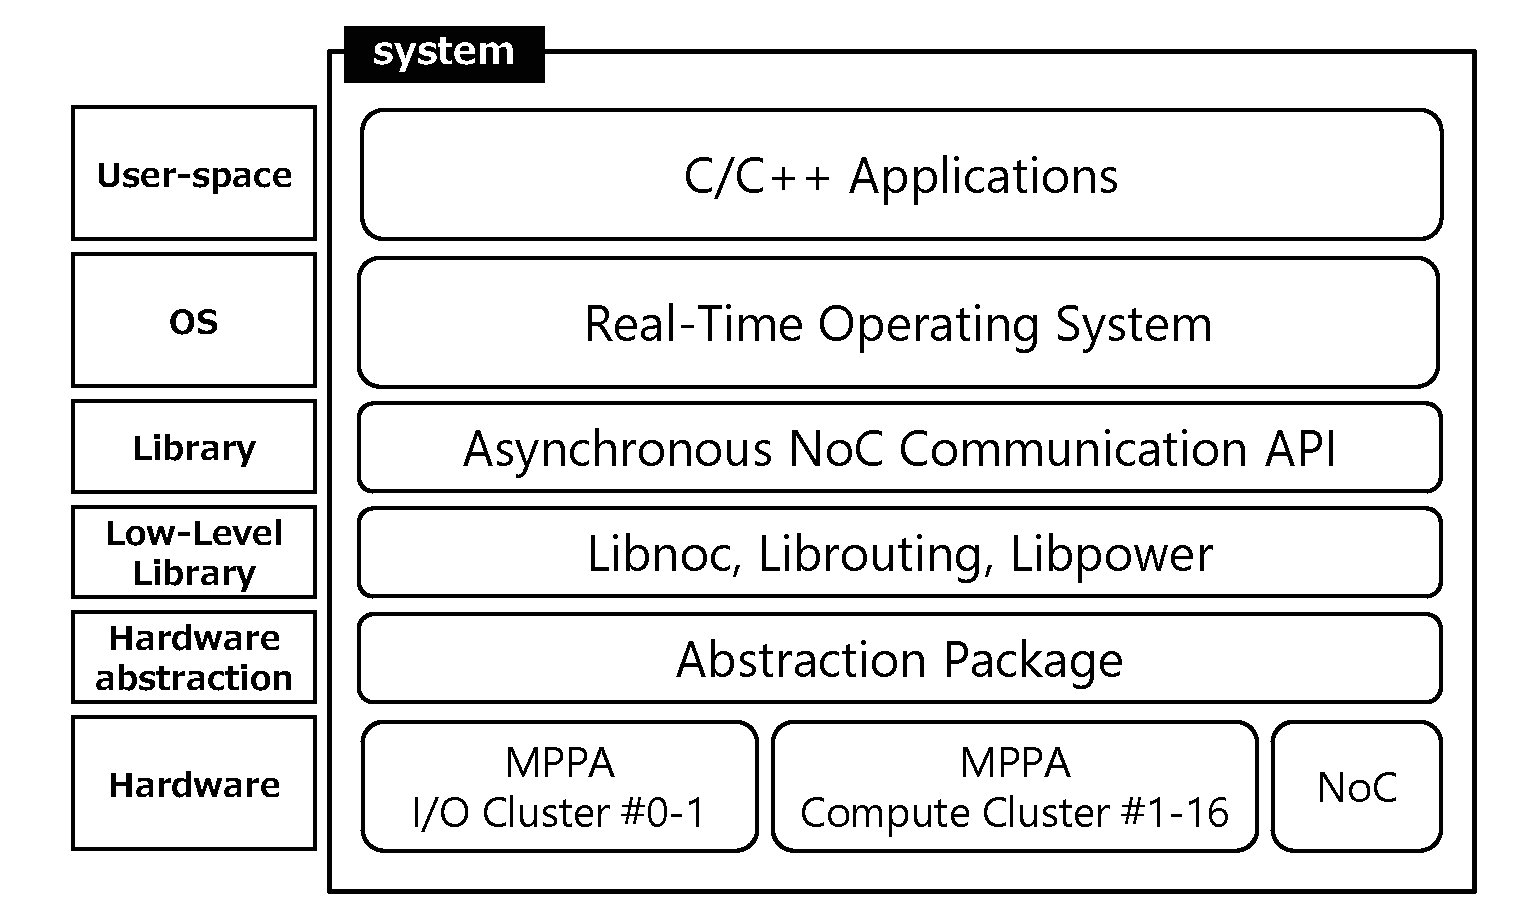
\includegraphics[width=0.7\linewidth]{../figure/softwarestack.eps}   
  \caption{\label{fig:software_stack}
    The software stack of Kalray MPPA-256.}     
\end{figure*}

The software stack used for Kalray MPPA-256 is composed of a hardware abstraction layer, a library layer, an OS, and a user application.  
Fig. \ref{fig:software_stack} shows the software stack used for Kalray MPPA-256 in the present work.
The Kalray system is an extensible and scalable array of computing cores and memory.
With respect to the scalable computing array of the system, it is possible to map several programming models or runtimes such as Linux, a real-time operating system, POSIX API, OpenCL, and OpenMP.
Each layer is described in detail.

In the hardware abstraction layer, an abstraction package abstracts hardware of a CC, an IOS, and NoC.
\comment{1-15} % The abstraction package serves as a system that does not provide any services.
The hardware abstraction is responsible for partitioning hardware resources and controlling access to the resources from the user-space operating system libraries.
\comment{1-16} 
% Additionally, the abstraction package retrieves resources allocated to a partition at any time.
The abstraction sets-up and controls inter-partition communications as a virtual machine abstraction layer.
The hardware abstraction runs on the dedicated RM core.
All the services are provided commonly by an operating system (e.g., virtual memory and schedule) that must be provided by user-space libraries.
% Consequently, each runtime or operating system implements its own services that are optimized to specific needs.
% This is because each programming model or runtime involves different requirements.
A minimal kernel avoids wastage of resources and mismatched needs.

In a low-level library layer, the Kalray system also provides mppa\_noc and mppa\_routing for handling NoC.
Additionally, NoC features such as routing and quality of service are set by the programmer.
mppa\_noc allows direct access to memory mapped registers for their configurations and uses.
This library is designed to cause minimum CPU overhead and also serves as a minimal abstraction for resource allocation.
% Librouting offers a minimal set of functions that can be used to route data between any clusters of the MPPA including unicast (one target) modes or multicast (multiple targets) modes.
mppa\_routing offers a minimal set of functions that can be used to route data between any clusters of the MPPA.
Routing on the network is conducted statically with its own policy.
In addition, mppa\_power enables spawning and waiting for the end of execution of other clusters.

\comment{1-17}
% Routing on the torus network is statically conducted with its own policy.
% The Libpower enables spawning and waiting for the end of execution of a remote cluster.

\subsection{Operating System}
\label{sec:operating_system}
Several operating systems support the abstraction package in the OS layer.
It is difficult for numerous cores such as MPPA to support previous operating systems for single/multicore(s) owing to problems involving parallelism and cache coherency \cite{Wentzlaff2009FOS}, \cite{schupbach2008embracing}.
Here, the following real-time operating systems (RTOSs) supporting MPPA are introduced:

\begin{itemize}
  \setlength{\leftskip}{-5mm}    
  \item \textbf{RTEMS}: Real-Time Executive for Multiprocessor Systems (RTEMS) is a full-featured RTOS prepared for embedded platforms.
  RTEMS supports several APIs and standards, and most notably supports the POSIX API.
  The system provides a rich set of features, and an RTEMS application is mostly a regular C or C++ program that uses the POSIX API.
  \comment{1-18}
  RTEMS runs on the IOC except for the CC.
  
  \item \textbf{NodeOS}: On the CC, the MPPA cluster operating system utilizes a runtime called NodeOS.
  The OS addresses the need for a multicore OS to conform to the maximum possible extent to the standard POSIX API.
  The NodeOS enables a user code by using the POSIX API to run on PEs on the CC.
  First, NodeOS runtime starts on PE0 prior to calling the user main function.
  Subsequently, \texttt{pthread} is called on other PEs.
  
  \item \textbf{eMCOS}: On both CCs and IOSs, eMCOS provides minimal programming interfaces and libraries.
  Specifically, eMCOS is a real-time embedded operating system developed by eSOL (a Japanese supplier for RTOSs) and is the first commercially available many-core RTOS for use in embedded systems.
  The OS implements a distributed microkernel architecture.
  This compact microkernel is equipped with only minimal functions.
  The eMCOS enables applications to operate priority based message passing, local thread scheduling, and thread management on IOSs as well as CCs.
\end{itemize}

RTMES and NodeOS are provided by Kalray and eMCOS is released by eSOL.

\subsection{NoC Data Transfer Methods}
\label{sec:data_transfer_methods}
\comment{TBD: 1-19: To be fully refleshed, Add setup and approach}
In this section, data transfer methods in MPPA-256 are explained.
For scalability purposes, MPPA-256 accepts a clustered architecture that avoids frequent memory contention between numerous cores, and it also accepts clustered architectures in which each cluster contains its own memory.
Sixteen cores are packed as a cluster sharing 2 MB memory (SMEM), as shown in Fig. \ref{fig:cc_architecture}.
This avoids frequent memory contention due to having numerous cores and helps in increasing the number of cores.
However, the architecture constrains memory that can be directly accessed by the cores.
Communicating with cores outside the cluster requires transferring data between clusters through the D-NoC with NoC interfaces.

In a low-level layer, each cluster on MPPA-256 contains hardware for a NoC interface, which has DMA units accounting for data receiving and sending: an Rx, Tx, and UC interfaces.

An Rx interface exists on the receiving side to receive data with DMA.
It is necessary to allocate a D-NoC Rx resource and configure the Rx to wait to receive the data.
A DMA in a NoC interface contains 256 D-NoC Rx resources.

Two interfaces, the Tx interface and the UC interface as explained in Sections \ref{sec:ios} and \ref{sec:cc},
are present with respect to the sending side for users to send data between clusters.
The UC is a network processor that is programmed to set threads to send data in DMA.
The UC executes programmed patterns and sends data through the D-NoC without a PE or an RM.
The UC interface results in higher data transfer throughput compared to the direct activation of the Tx interface.
However, a DMA in a NoC interface contains only eight D-NoC UC resources.
Both interfaces use a DMA engine to access memory and copy data.
Regardless of whether a UC interface is used, it is necessary to allocate a D-NoC Tx resource and configure the Tx to send data.
Additionally, it is necessary to allocate and configure D-NoC UC resources, if a UC interface is used.

Application developers have several choices to transfer data on D-NoC between clusters.
Kalray provides mppa\_noc and mppa\_async libraries and eMCOS provides two kinds of message APIs.
Table \ref{tb:comparison_noc} compares features of each method.
Specifications are different for each method, and it is necessary to use properly according to the purpose.
In an internal implementation, all methods are based on mppa\_noc.
mppa\_noc is low-level NoC communication library and provides users interfaces to handle DMA resources such as an Rx, Tx and UC interfaces for NoC data transfer.
Each method which application developers are able to use is described in detail as below.

\begin{table*}[!htbp]
  \caption{\label{tb:comparison_noc}
    Comparison of NoC Data Transfer Methods}
  \centering
  \scriptsize	                    % text size
  \tabcolsep = 1.5mm              % side-margin in column
  \begin{tabular}{c|ccccccc}
    \hline
    & \multirow{2}{*}{Provider} & \multirow{2}{*}{Model} & Resource & Buffer & DMA & Equality of \\
    & & & Management & Allocation & Type & IOC and CC \\
    \hline
    \hline
    mppa\_noc & Kalray & send/receive & self & user-space & Tx/UC & equal \\
    mppa\_async & Kalray & read/write & auto & user-space & Tx & non-equal\\
    eMCOS message & eSOL & send/receive & auto & kernel-space & Tx & equal \\
    eMCOS session message & eSOL & send/receive & auto & user-space & UC & equal \\
    \hline
  \end{tabular}
\end{table*}

\begin{itemize}
  \setlength{\leftskip}{-5mm}
  \item \textbf{mppa\_noc}:
  \item \textbf{mppa\_async}:
  \item \textbf{eMCOS message}:
  \item \textbf{eMCOS session message}:
\end{itemize}


\chapter{Proposed Framework}
\label{chap:proposed_framework}

\begin{figure*}[!htbp]
  \centering
  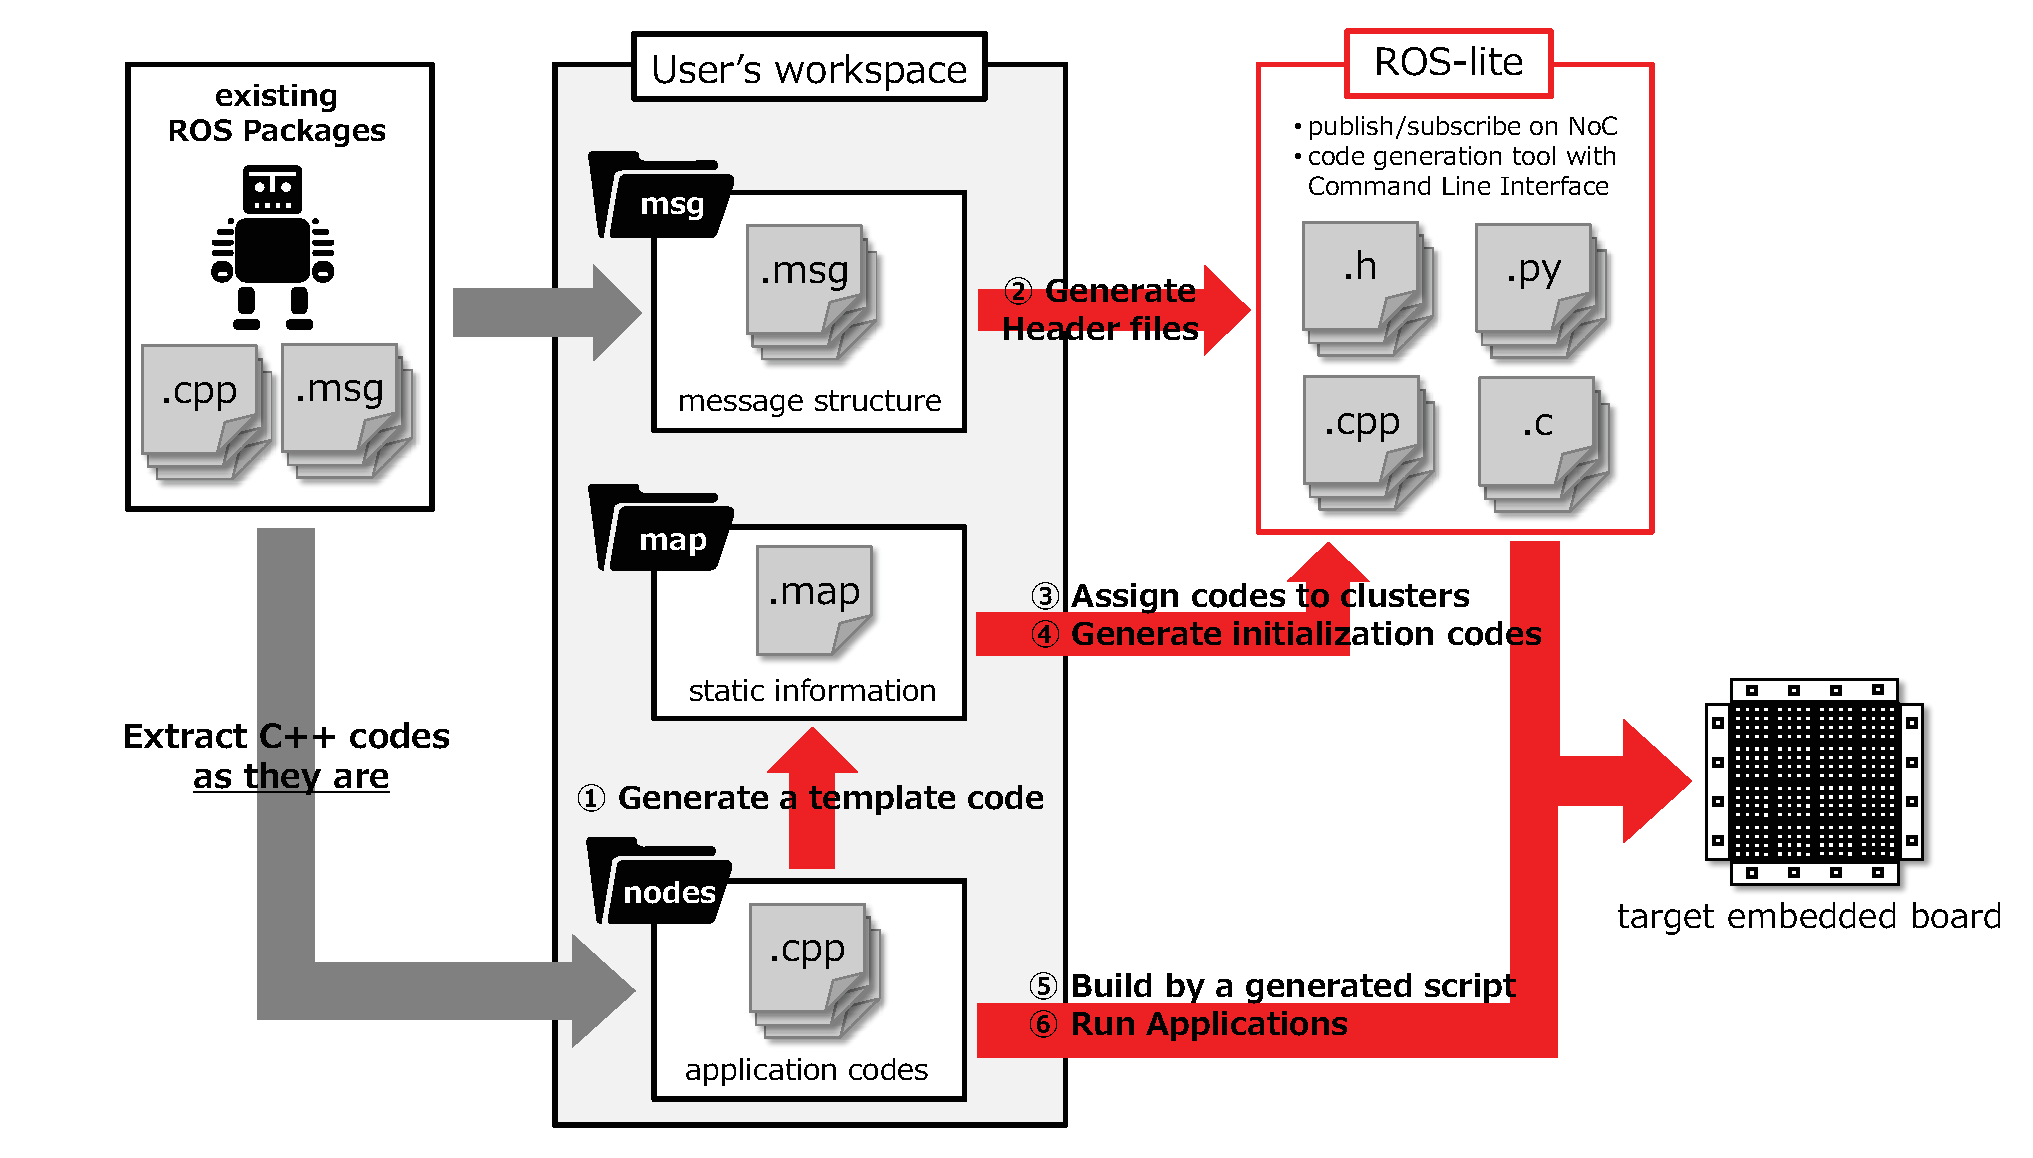
\includegraphics[width=0.7\linewidth]{../figure/roslite/system_model.eps}
  \caption{\label{fig:rosl_system_model}
    Development flow of ROS-lite framework.}
\end{figure*}

The proposed framework, ROS-lite, is structured communications layer for efficient development on many-core platforms.
Although existing ROS has been being rapidly developed and widely used, the ROS does not support NoC communication and embedded requirement such as RTOS and limited memory on embedded platforms.
ROS-lite is a solution for these challenges and provides a development environment in which ROS nodes run on each core on many-core platforms and communicate with each other.
By enabling and extending numerous existing ROS applications, transporting and new development on embedded platforms are made much more efficient.
(For more information of ROS basic, please refer to Apendix A: Robot Operating System (ROS).)
Additionally, being based on existing ROS framework, ROS-lite has potential to communicate external ROS nodes on other platform.
Design of ROS-lite can enhance efficient development on heterogeneous computing platforms.
In this paper, we target eMCOS as RTOS and MPPA-256 as an embedded many-core platform.

\section{ROS-lite Toolchain}
\label{sec:toolchain}

\begin{figure*}[!htbp]
  \tabcolsep = 0.5mm              % side-margin in column
  \begin{tabular}{cc}
    \begin{minipage}[!htbp]{0.59\textwidth}
      \centering
      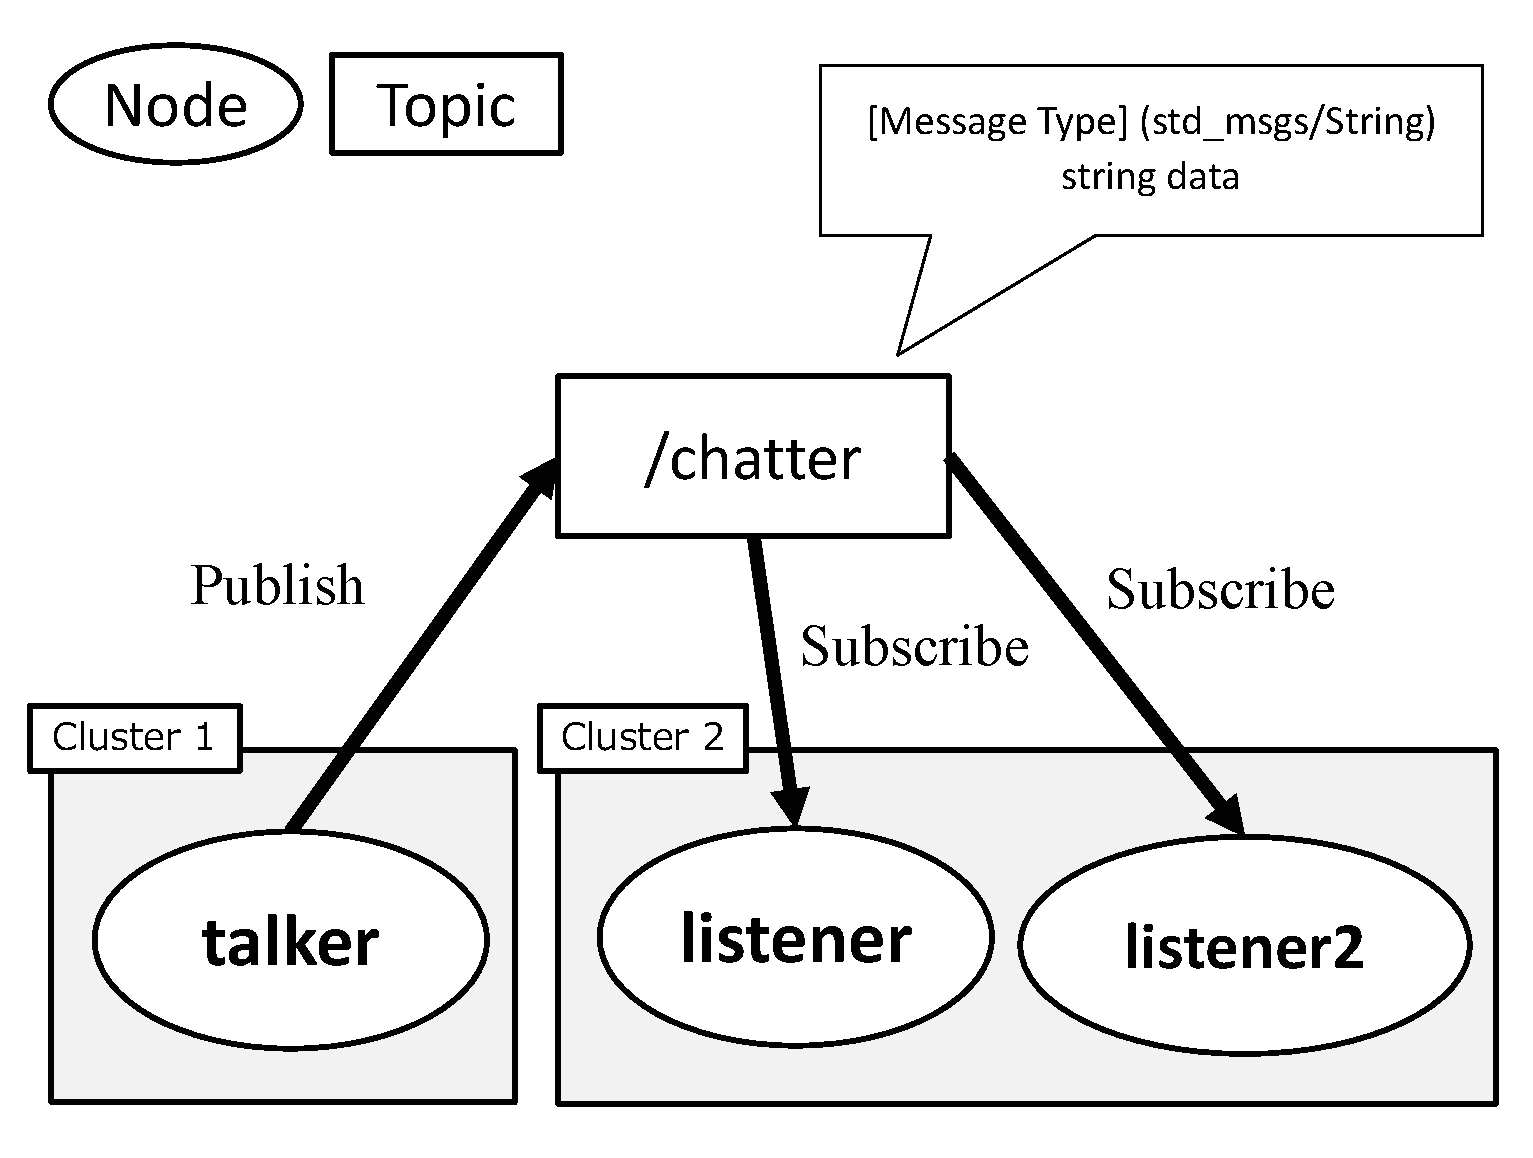
\includegraphics[width=0.85\linewidth]{../figure/roslite/example.eps}
      \caption{The publish/subscribe model in ROS-lite.}
      \label{fig:rosl_example}
    \end{minipage}
    &
    \begin{minipage}[!htbp]{0.39\textwidth}
      \lstinputlisting{../code/roslite_map_two_listenres.map}
      \caption{Map file Description.}
      \label{code:map_file}
    \end{minipage}
  \end{tabular}
\end{figure*}

This section describes a system model and a proposed framework used to run ROS nodes on an embedded many-core platform.
The system architecture of ROS-lite is shown in Fig. \ref{fig:rosl_system_model}.
ROS-lite can run application codes written as ROS nodes.
We assume that application codes following ROS manner are written in C++.
Application developers can extract source codes (application codes and message structure files) from existing ROS packages them as they are.
For task mapping, developers edit an map file (\texttt{.map}) and assign ROS nodes to the clusters on many-core platforms.
All developers have to do for modification of task mapping is editing map file.
ROS nodes as processes on cores are described as publish/subscribe model, following message structures defined in message files (\texttt{.msg}).
ROS nodes can communicate with each other via either innner-cluster or inter-cluster communications.
While these cores do communications via shared memory in innner-cluster, the cores do communications via NoC in inter-cluster.

Our framework provides code generation and build system by command line interface for efficient development.
First, in \textcircled{\scriptsize 1} of Fig. \ref{fig:rosl_system_model}, a template of a map file (\texttt{.map}) is generated from application source codes.
The map file (\texttt{.map}) contains node name, assigned cluster, information of topics published and subscribe to.
These descriptions except for assigned cluster number is able to be interpreted from ROS nodes so that we provide code geraration for template codes.
Application developers can focus on the number of assigned cluster.
Second, in \textcircled{\scriptsize 2} of Fig. \ref{fig:rosl_system_model}, header files defining message structure are generated from message files (\texttt{.msg}) as an original ROS does.
Note that generated header file has been made lighter because the part required by ROS-lite is generated.
This code generation part is based on an original ROS's script and message files (\texttt{.msg}) can be described in the same manner.
Developers do not have to modify message files (\texttt{.msg}) at all.
Third, in \textcircled{\scriptsize 3} and \textcircled{\scriptsize 4} of Fig. \ref{fig:rosl_system_model}, initialization codes of launching processes of ROS nodes are generated from a map file (\texttt{.map}).
ROS nodes are automatically launched as processes scheduled by RTOS on user-assigned clusters on embedded platforms.
Application developers do not have to write codes except for ROS nodes.
Finally, in \textcircled{\scriptsize 5} of Fig. \ref{fig:rosl_system_model}, a build script is generated from a user-defined map file (\texttt{.map}).
Source codes of ROS nodes are separately built in each user-assigned cluster because the executable files are loaded into separate memories for each cluster.
This building process is conducted witd generated build script.
There is no need to modify build script each time developers change task mapping by modification of the map file (\texttt{.map}).
All codes of ROS nodes are allocated in a same directory and are automatically built in each user-assigned cluster.

We give a simple example for explaination of ROS-lite framework.
One node publishes a \emph{chatter} topic and two nodes subscribe to the topic as shown in \ref{fig:rosl_example}.
Messages in the \emph{chatter} topic are defined as string type named \emph{data}.
The publisher node is launched in \emph{cluster 1} and two subscriber node in \emph{cluster 2}, as described in assigned cluster number in the map file (\texttt{.map}) of Fig. \ref{code:map_file}.
Application developers can change node mapping by modification of the field of cluster number.
Information of topics in map file (\texttt{.map}) is used for initialization of the relationship between the topics and the nodes so that ROS-lite conducts the process of matching the nodes to communicate by topic names.
These field of the node name and topic information are generated from source codes of ROS nodes, and initialization codes of the node relationship for ROS-lite are generated from the map file (\texttt{.map}).
Note that the field of assigned cluster number has to be filled by developers.

\section{Design and Implementation}
\label{sec:design_and_implementation}
% To make existing ROS runing on many-core platforms, \ref{code:map_file}, \ref{fig:rosl_example} hoge.

\memo{design choice:}
\memo{assign cluster not core affinity}
\memo{why? scheduled by eMCOS. mapping is future work and out of scope in this paper.}
\memo{No master as searver. static initialization with map file}
\memo{why? avoid single point failure}
\memo{why? for analysis of real-time requirement in future work}
\memo{why? The dynamic node set change at runtime is rare in embedded system}


\begin{figure}[!htbp]
  \centering
  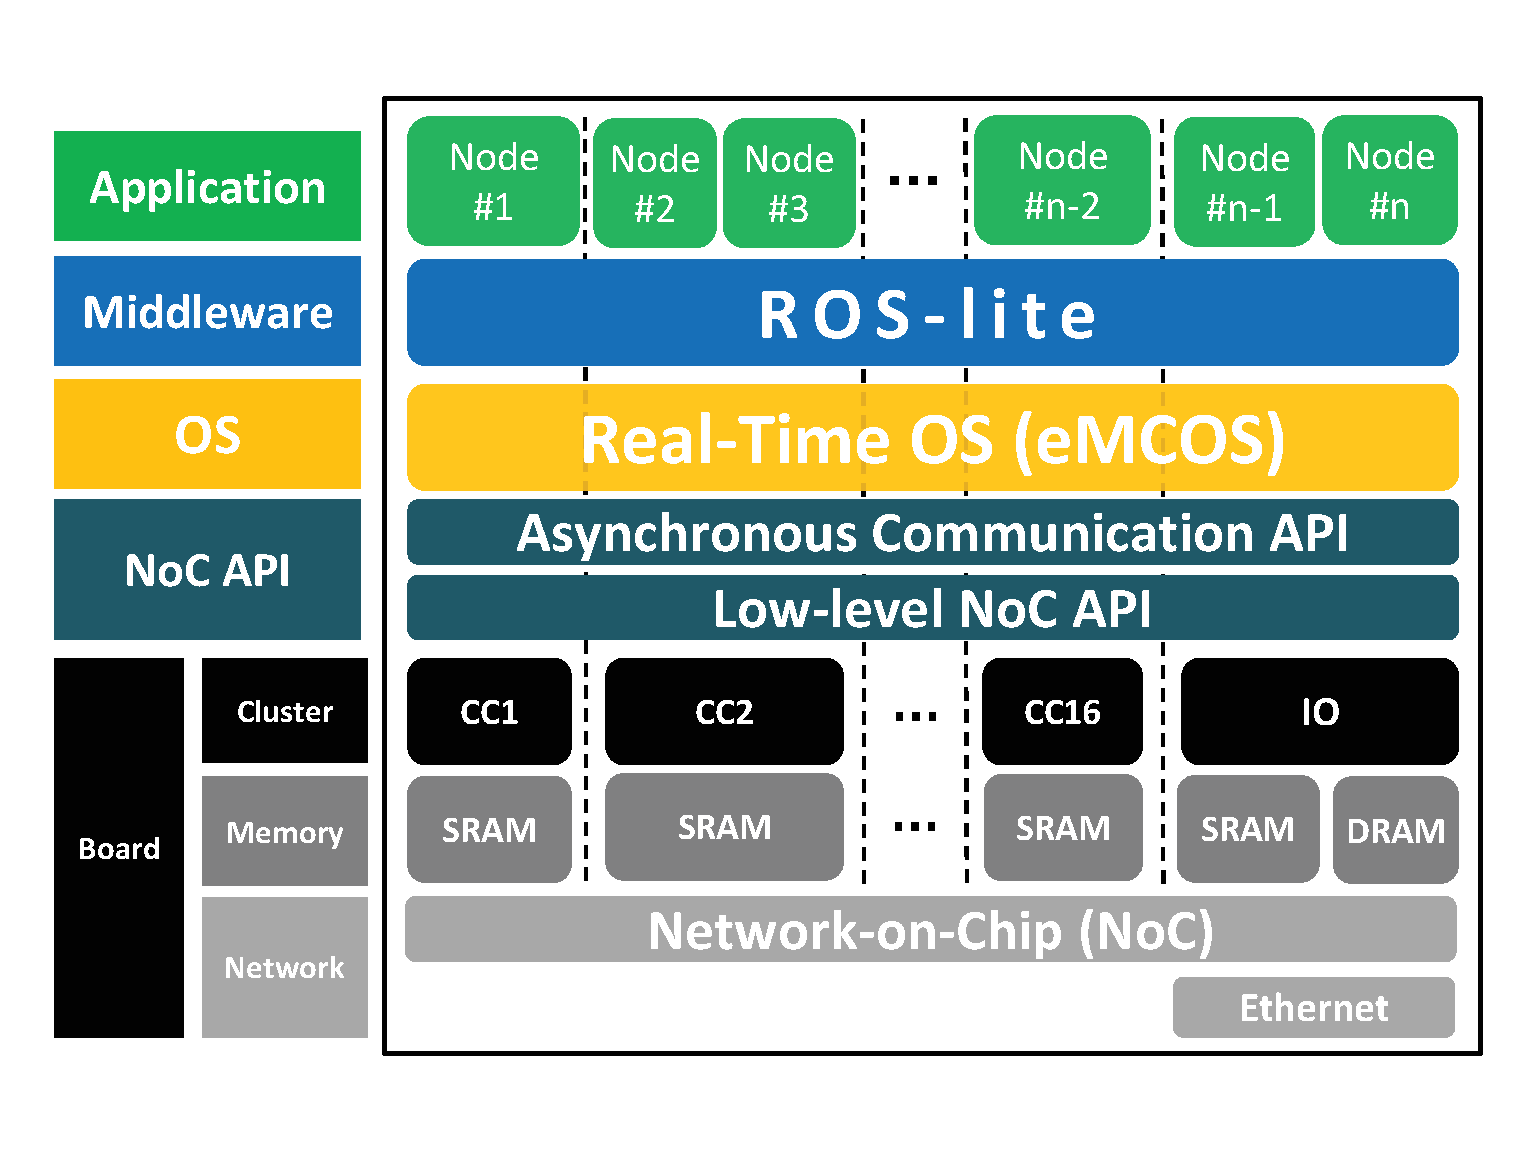
\includegraphics[width=0.7\linewidth]{../figure/roslite/software_stack.eps}
  \caption{\label{fig:rosl_software_stack}
    System stack of ROS-lite on a many-core platform.}
\end{figure}


\chapter{Evaluations}
\label{chap:evaluations}
First, this section involves examining two types of evaluations: a D-NoC data transfer evaluation in which latency characteristics of interfaces and memory type are explored and a matrix calculation evaluation that demonstrates the parallelization potential of the MPPA-256 and its memory access characteristics.
Subsequently, we conduct a practical self-driving application to examine the practicality of NUMA many cores.
% Finally, we arrange lessons learned from above evaluations.
The following evaluations are all conducted on real hardware boards with eMCOS.

\section{D-NoC Data Transfer}
\label{sec:dnoc_eval}

\subsection{Situations and Assumptions}
\label{sec:situations_and_assumptions2}

\begin{figure}[!htbp]
  \centering
  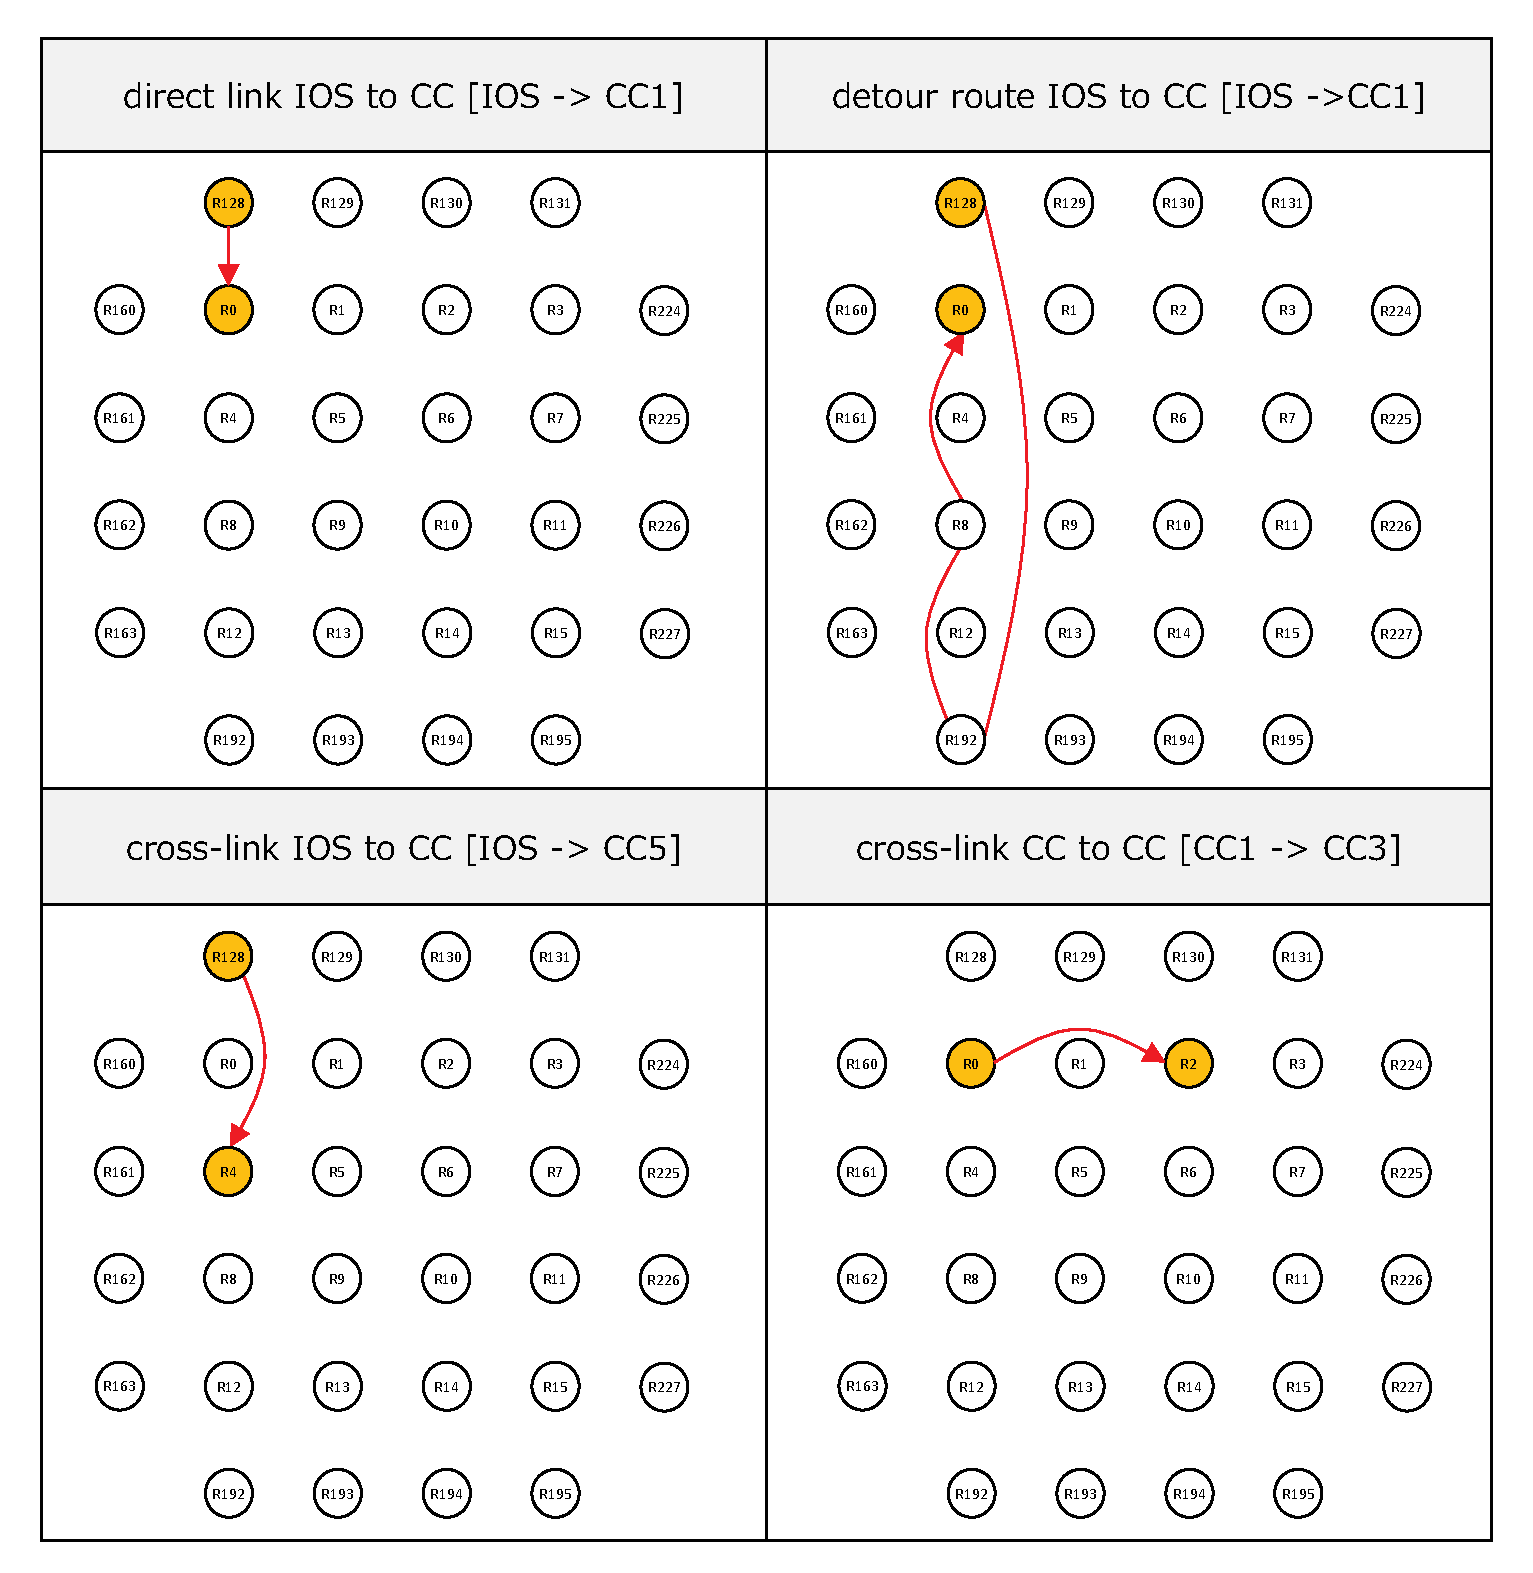
\includegraphics[width=0.5\linewidth]{../figure/noc_routes_old.eps}
      \caption{\label{fig:noc_routes}
    Four D-NoC routes used in the evaluation.}
\end{figure}

This evaluation involves clarifying end-to-end latency by considering the relation among interfaces (Tx or UC), routing on NoC, and memory type (DDR or SMEM).
This is achieved by preparing four routes as shown in Fig. \ref{fig:noc_routes}.
The routes on the D-NoC map (Fig. \ref{fig:noc_map}) contain various connections between routers, a direct link, a cross-link, and a flying link.
With respect to the case of routes from the IOS routers to the CC routers, transmitted data are allocated in the DDR or IO SMEM.
The CC includes only the SMEM as shown in Fig. \ref{fig:cc_architecture}.
% A low-level library is directly used to transfer data with D-NoC.
The transferred data correspond to 100 B, 1 KB, 10 KB, 100 KB, and 1 MB.
The buffers are sequentially allocated in DDR or SRAM (IO SMEM or CC SMEM).
The capacity of the CC SMEM is 2 MB, and thus it is assumed that the appropriate communication buffer size is 1 MB.
Given this assumption, the other memory area corresponds to the application, libraries, and an operating system.
End-to-end latencies are measured 1,000 times in numerous situations as shown in Figs. \ref{fig:DDR_tx}, \ref{fig:DDR_uc}, and \ref{fig:IO_SMEM_tx}, and boxplots are obtained, as depicted in Figs. \ref{fig:IO_SMEM_uc}, \ref{fig:tx_uc_log}, and \ref{fig:tx_uc}.
In the evaluation setting, we minimize traffic conflicts to focus on the relation between end-to-end latency and routing on NoC.

\subsection{Influences of Routing and Memory Type}
\label{sec:routing_and_memory}

\comment{1-20, 1-21}
Data transfer latencies between an IOS and a CC are influenced little by routing.
This involves preparing two interfaces (Tx and UC), three routes (direct link, cross-link, and detour route), and two memory locations in which the transferred data are allocated.
As shown in Figs. \ref{fig:DDR_tx}, \ref{fig:DDR_uc}, \ref{fig:IO_SMEM_tx}, and \ref{fig:IO_SMEM_uc}, 
end-to-end latency scales exhibit a linear relation with data size, and there are no significant differences between the three routes with respect to data transfer latency.
This result is important in a torus topology NoC because the number of minimum steps exceeds that in a mesh topology. 
It is observed that queuing in NoC routers and hardware distance on a NoC are not dominant factors for latency.
The router latency, the time taken in transmitting and receiving transactions in an RM, exceeds those of other transactions.
Additionally, it is briefly recognized that the speed of the UC exceeds that of the Tx.
The data are arranged as shown in Figs. \ref{fig:tx_uc_log} and \ref{fig:tx_uc} to facilitate a precise analysis with respect to the interface and memory location.
In those figures, only the cross-link from the IOS to CC5 is accepted because routes do not influence latency.
To facilitate intuitive recognition, two kinds of figures are arranged: a logarithmic and a linear axis.

In the Tx interface, DDR causes a large increase in latency.
The time taken by the DDR is twice that of the IO SMEM as shown in Fig. \ref{fig:tx_uc_log}.
This is due to the memory access speed characteristics of DRAM and SRAM.
In the Tx interface, it is necessary for an IO core on an IOS to operate the DMA in the IOS NoC interface.
This is attributed to the fact that the core is involved in processing.
The speed of the data transfer latency between CCs exceeds that between an IOS and a CC.
This result indicates that the MPPA-256 is optimized for communication between the CCs.

With respect to the UC interface, the latency is not significantly affected by the location at which the transferred buffer is allocated (i.e., DDR or SMEM).
Similar latency characteristics are observed in Fig. \ref{fig:tx_uc_log}.
In the case of the UC interface, an IO core on the IOS does not involve a DMA transaction.
A UC in the NoC interface executes a programmed thread sending data.
This evaluation result suggests that the slow access speed of the DDR is not significant in the case of the UC.
In a manner similar to that of the Tx interface, the speed of the data transfer latency between CCs exceeds that between an IOS and a CC.

\clearpage

\begin{figure*}[!htbp]
  \tabcolsep = 0.5mm              % side-margin in column
  \begin{tabular}{cc}
    % \setcounter{figure*}{9}
    \begin{minipage}[!htbp]{0.49\textwidth}
      \includegraphics[width=1.0\linewidth]{../../R/mppa/graph/eps/BoxPlot_DDR_tx.eps}
      \caption{Data transfer with Tx from IO DDR to CC.}
      \label{fig:DDR_tx}
    \end{minipage}
    &
    % \setcounter{figure*}{11}
    \begin{minipage}[!htbp]{0.49\textwidth}
      \includegraphics[width=1.0\linewidth]{../../R/mppa/graph/eps/BoxPlot_DDR_uc.eps}
      \caption{Data transfer with UC from IO DDR to CC.}
      \label{fig:DDR_uc}
    \end{minipage}
  \end{tabular}
\end{figure*}

\begin{figure*}[!htbp]
  \tabcolsep = 0.5mm              % side-margin in column
  \begin{tabular}{cc}
    % \setcounter{figure*}{9}
    \begin{minipage}[!htbp]{0.49\textwidth}
      \includegraphics[width=1.0\linewidth]{../../R/mppa/graph/eps/BoxPlot_IO_SMEM_uc.eps}
      \caption{Data transfer with UC from IO SMEM to CC.}
      \label{fig:IO_SMEM_tx}
    \end{minipage}
    &
    % \setcounter{figure*}{11}
    \begin{minipage}[!htbp]{0.49\textwidth}
      \includegraphics[width=1.0\linewidth]{../../R/mppa/graph/eps/BoxPlot_IO_SMEM_uc.eps}
      \caption{Data transfer with UC from IO SMEM to CC.}
      \label{fig:IO_SMEM_uc}
    \end{minipage}
  \end{tabular}
\end{figure*}

\begin{figure*}[!htbp]
  \tabcolsep = 0.5mm              % side-margin in column
  \begin{tabular}{cc}
    % \setcounter{figure*}{9}
    \begin{minipage}[!htbp]{0.49\textwidth}
      \includegraphics[width=1.0\linewidth]{../../R/mppa/graph/eps/BoxPlot_Tx_vs_UC_log.eps}
      \caption{Data transfer with Tx/UC (logarithmic axis).}
      \label{fig:tx_uc_log}
    \end{minipage}
    &
    % \setcounter{figure*}{11}
    \begin{minipage}[!htbp]{0.49\textwidth}
      \includegraphics[width=1.0\linewidth]{../../R/mppa/graph/eps/BoxPlot_Tx_vs_UC.eps}
      \caption{Data transfer with Tx/UC (linear axis).}
      \label{fig:tx_uc}
    \end{minipage}
  \end{tabular}
\end{figure*}

\clearpage

\section{Matrix Calculation}
\label{sec:martix_eval}

\subsection{Situations and Assumptions}
\label{sec:situations_and_assumptions1}

\begin{figure*}[!htbp]
  \centering
  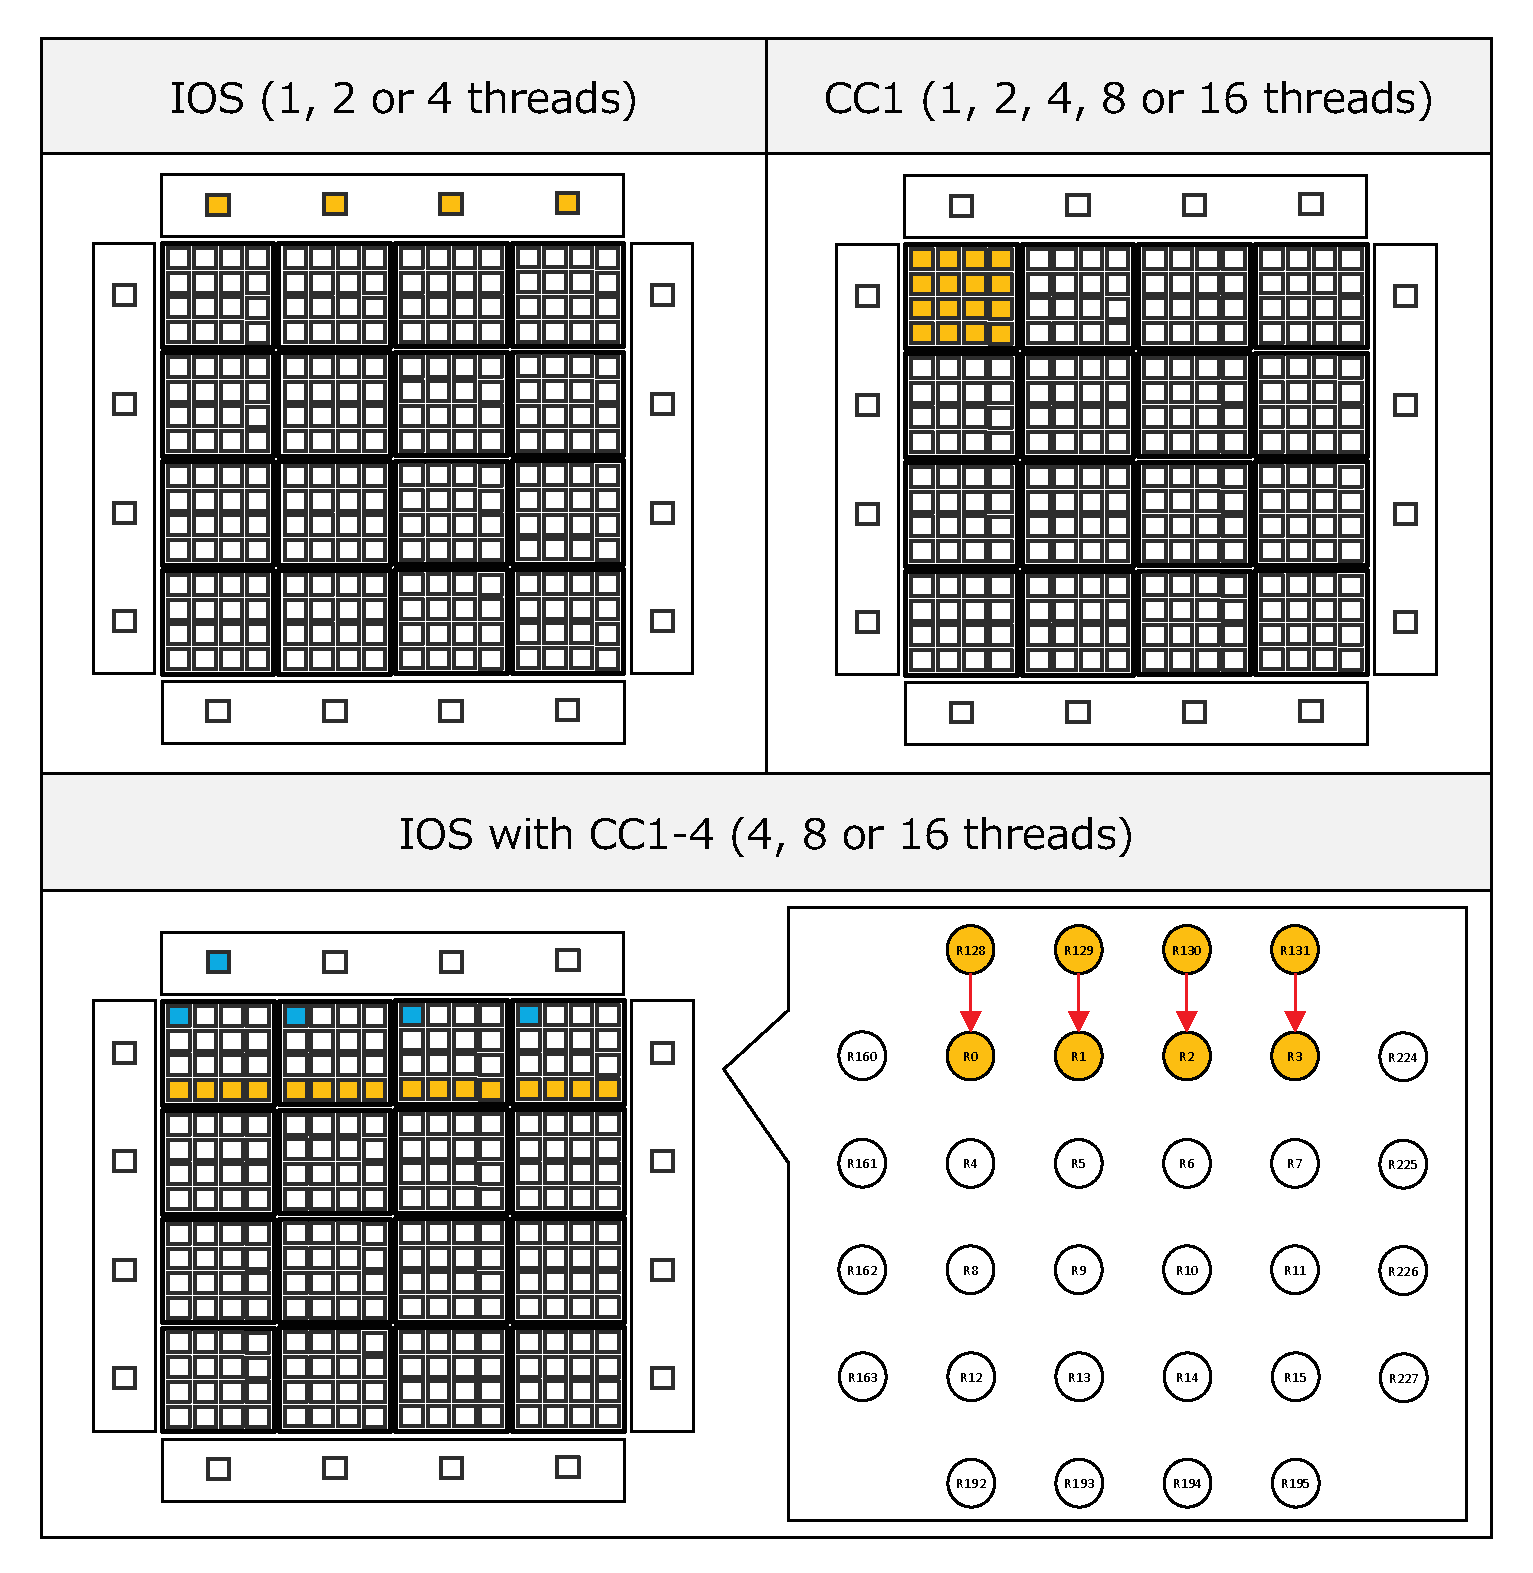
\includegraphics[width=0.5\linewidth]{../figure/matrix_calculation.eps}
  \caption{\label{fig:mat_calc}
    Matrix calculation situations.}
\end{figure*}

In the evaluation, the matrix calculation time and parallelization potential of MPPA-256 are clarified.
Matrix calculations are conducted in an IOS and CCs.
Three computing situations are considered as shown in Fig. \ref{fig:mat_calc}.
The first situation involves computing in the IOS where four cores are available.
To analyze memory access characteristics, a matrix buffer is allocated in the IO DDR and SMEM.
The second situation involves computing in a CC in which 16 cores are available.
The third situation involves offload-computing using an IOS and four CCs.
Parallelized processing is executed with four CCs and SMEMs.
A few cores in the IOS and CC manage the parallelized transaction.
The method can handle large amount of data in which one cluster is not sufficient, because buffer capacity is not limited to 2 MB in the SMEM.
Parallelized processing and the total capacity of the SMEM are superior to single IOS or CC computations. 
With respect to the IOS, the application can handle large capacity data only in the DDR.
However, in this method, distributed memories are used to deal with large capacity data in the SMEM.
Thus, it is necessary for IOS and CC cores to access matrix buffers without cache to avoid cache coherency difficulties.
To facilitate faster data transfer, a portion of the matrix buffer is transmitted in parallel as shown in Fig. \ref{fig:mat_calc}.

Matrix calculation time is analyzed with parallelization and memory allocation.
Additionally, the influences of a cache are analyzed because cache coherency is an important issue in many-core systems.
There are several cases in which applications must access specific memory space without a cache because MPPA does not guarantee cache coherency between PEs.
With respect to the given assumptions, the maximum total buffer size is 1 MB, and thus three matrix buffers are prepared, each of size 314 KB.
Matrix A and Matrix B are multiplied, and the result is stored in Matrix C.
The total for the three matrices is set as approximately 1 MB.
We assume that the remainder of the SMEM (1 MB) is occupied with system software and applications in the CC.

\subsection{Influences of Cache and Memory Type}
\label{sec:cache_and_memory}
First, matrix calculation time with the cache in the IOS and CC is depicted in Fig. \ref{fig:mat_calc_cache}.
There are almost no differences between the IO DDR, IO SMEM, and CC SMEM due to the cache.
A 128 KB data cache in the IOS works well and compensates for the DDR delay.
Additionally, it is observed that calculation time scales exhibit a linear relation with the number of threads.
This corresponds to ideal behavior with respect to parallelization.

Second, matrix calculation time without a cache in the IOS and CC is shown in Fig. \ref{fig:mat_calc_uncache}.
The absence of a cache, results in a fourfold increase in the DDR and a large difference arises with respect to the SMEM.
Another notable result is that calculation speed in the CC SMEM exceeds that of the IO SMEM.
This characteristic is hidden in the calculation with the cache.
The computing cores physically involve the same cores in the IOS and CC, and thus it is considered that the characteristics and physical arrangement of the SMEM exert a significant effect.
This is an interesting result since there is a large difference that cannot be ignored.
It is also observed that calculation time exhibits a linear relation with the number of threads.
Furthermore, in the CC SMEM, the calculation speed without the cache exceeds that with cache.
This result is contrary to intuition, and a cache line problem is conceivable.
When a small data cache (8 KB) in a PE of the CC does not function adequately and an application always misses the cache, memory access will pay the time for a noncached data access and the cost to refill the cache line.
As a result, the memory access speed without the cache exceeds that with it.

\clearpage

\begin{figure*}[!htbp]
  \centering
  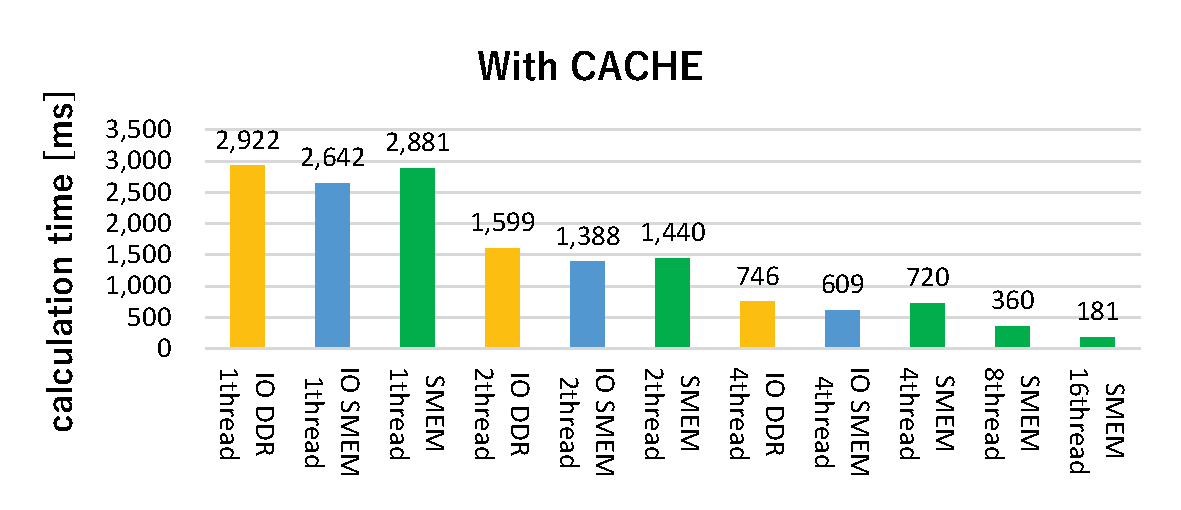
\includegraphics[width=.9\linewidth]{../figure/BarGraph_matrix_with_cache.eps}
  \caption{Matrix calculations in IOS and CC with cache.}
  \label{fig:mat_calc_cache}
\end{figure*}

\begin{figure*}[!htbp]
  \centering
  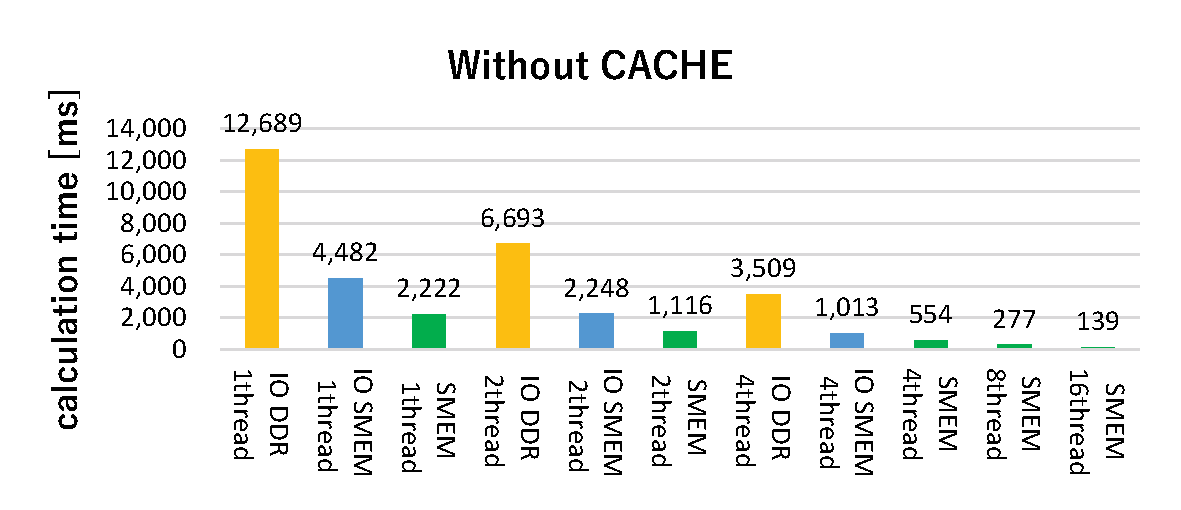
\includegraphics[width=.9\linewidth]{../figure/BarGraph_matrix_without_cache.eps}
  \caption{Matrix calculations in IOS and CC without cache.}
  \label{fig:mat_calc_uncache}
\end{figure*}

\subsection{Four CCs' Parallelization}
\label{sec:four_CCs}
Finally, matrix calculation with offload-computing in an IOS and CCs is shown in Figs. \ref{fig:mat_calc_offload_314} and \ref{fig:mat_calc_offload_640}.
In this case, it is assumed with respect to the calculation of large matrices that the total capacity exceeds 1 MB.
The offloading result is compared with the IO DDR (cached) owing to the aforementioned assumption.
The aggregate calculation is obtained by offloading on the four CCs to perform a multiplication of a tile of Mat A and a tile of the transpose of Mat B.
This produces an overhead irrespective of the number of threads as shown in Figs. \ref{fig:mat_calc_offload_314} and \ref{fig:mat_calc_offload_640}.

However, the speed involved in offloading the result exceeds that of the IO DDR (cached).
The result indicates several important facts.
First, D-NoC data transfer produces little overhead latency.
Second, the speed of DMA memory access to DDR exceeds that of the IO core's memory access, even if target memory is allocated on the DDR.
In the offloading case, a DMA accesses matrix buffers on the DDR and transfers the buffers from the IO DDR to each CC SMEM.
Subsequently, PEs in the CC access matrix buffer the calculation without a cache.
The overhead of data transfer and DMA memory access is small, and thus parallel data transmission and distributed memory are practical in the case of MPPA-256.
The impact of offloading increases when the matrix is large as shown in Fig. \ref{fig:mat_calc_offload_640}.
Only a portion of the matrix is allocated in CCs, and thus it is possible to handle larger matrix buffers.

Additionally, 640 KB matrices are prepared, and matrix calculation are evaluated with offload-computing.
The speed of the offloading result exceeds that of the IO DDR result with respect to the 314 KB matrices in Fig. \ref{fig:mat_calc_offload_314}.
In these offloading evaluations, each CC concurrently transmits calculation results to the IOS.
\comment{1-22}
When Matrix C in which calculation results are stored is allocated in the DDR, the NoC router's FIFOs sometimes overflow and cause an error due to memory access delay of the DDR.
The transmission protocol would ideally be expected to prevent this error, and flow control is intended as future work for MPPA-256.
Currently, to avoid this error, Matrix C must be allocated in the IO SMEM.
Note that the above evaluation results when Matrix C is allocated in the DDR.


\begin{figure*}[!htbp]
  \tabcolsep = 0.5mm              % side-margin in column
  \begin{tabular}{cc}
    \begin{minipage}[!htbp]{0.49\textwidth}
      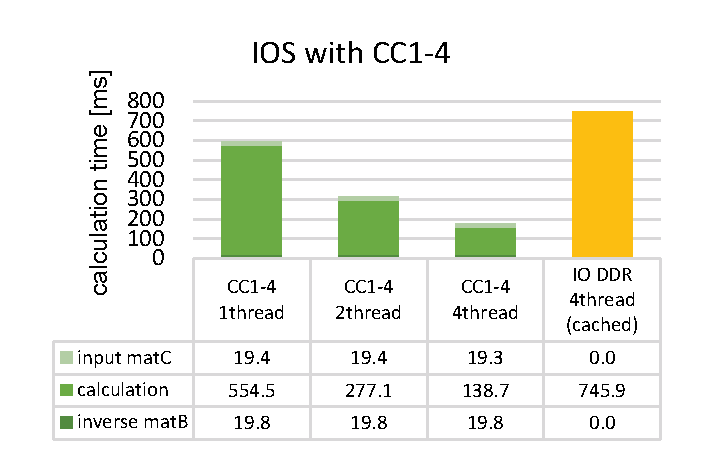
\includegraphics[width=0.9\linewidth]{../figure/BarGraph_matrix_with_CCs_314.eps}
      \caption{Matrix calculations with offload computing (314 KB matrix x 3).}
      \label{fig:mat_calc_offload_314}
    \end{minipage}   
    &
    % \setcounter{figure*}{11}
    \begin{minipage}[!htbp]{0.49\textwidth}
      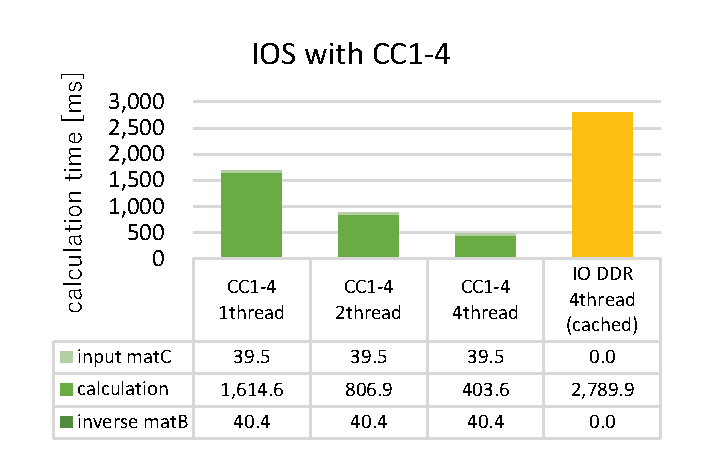
\includegraphics[width=0.9\linewidth]{../figure/BarGraph_matrix_with_CCs_640.eps}
      \caption{Matrix calculations with offload computing (640 KB matrix x 3).}
      \label{fig:mat_calc_offload_640}
    \end{minipage}
  \end{tabular}
\end{figure*}

\section{Practical Application}
\label{sec:practical_application}
This work adopts a portion of a self-driving system and this section demonstrates the parallelization potential of the MPPA-256.
We selected an algorithm for vehicle self-localization written in C++ in Autoware, open-source software for urban self-driving \cite{autoware}, and a parallelized part of it.
(Please refer to Apendix B: Autoware.)
The self-localization adopts the normal-distribution transform matching algorithm \cite{magnusson2009three} implemented in the Point Cloud Library \cite{pcl}.
A diagram depicting self-localization is shown in Fig. \ref{fig:ndt_matching_situation}.

% The self-localization algorithm is primarily divided into two processes: \emph{RadiusSearch} which searches for several nearest neighbor points for each query and calculates the distance, and \emph{Derivatives} which calculates the derivative to determine the convergence of the matching operation.
% As shown in Fig. \ref{fig:ndt_matching_situation}, 
% This evaluation parallelized \emph{Derivatives} onto 16 CCs and the remainder of the algorithm was executed on the IOS with its four cores.
% To parallelize \emph{RadiusSearch}, the algorithm of the nearest neighbor search needs to be redesigned because the data to be searched exceeds 1 MB.
% Redesigning this algorithm will be part of a future work.

The self-localization algorithm is composed primarily of the \emph{computeTransform} function which searches for several nearest neighbor points for each scan query and calculates a matching transformation.
This evaluation parallelized a part of \emph{computeTransform} onto 16 CCs and the remainder of the algorithm was executed in parallel on the IOS with its four cores.
To parallelize the remainder of \emph{computeTransform} in CCs, the algorithm of the nearest neighbor search must be redesigned because the data to be searched exceeds 1 MB.
Redesigning this algorithm is reserved for future work, and there is room for improvement through the parallelization potential of the MPPA-256.

As shown in Fig. \ref{fig:ndt_matching}, the evaluation of the parallelized self-localization algorithm indicates the average execution time for each convergence and demonstrates that the parallelization accelerates the \emph{computeTransform} process.
% Because the reduction of the execution time of \emph{computeTransform} involves reducing the number of loops for convergence, the execution times of \emph{RadiusSearch} and other parts are also shortened.
The query can be assumed to be 10 Hz in many automated driving systems.
Thus, this tuning successfully meets the deadline.
This parallelized algorithm was executed on simulated and real car experiments in our test course and worked successfully.
The steering, accelerator, and brake are automatically controlled based on the results of MPPA-256.
A demonstration video of the adaptation of the parallelized self-localization algorithm to Autoware on eMCOS can be seen at: https://youtu.be/wZyqF90c5b8  

\begin{figure*}[!htbp]
  \tabcolsep = 0.5mm              % side-margin in column
  \begin{tabular}{cc}
    \begin{minipage}[!htbp]{0.49\textwidth}
      \centering
      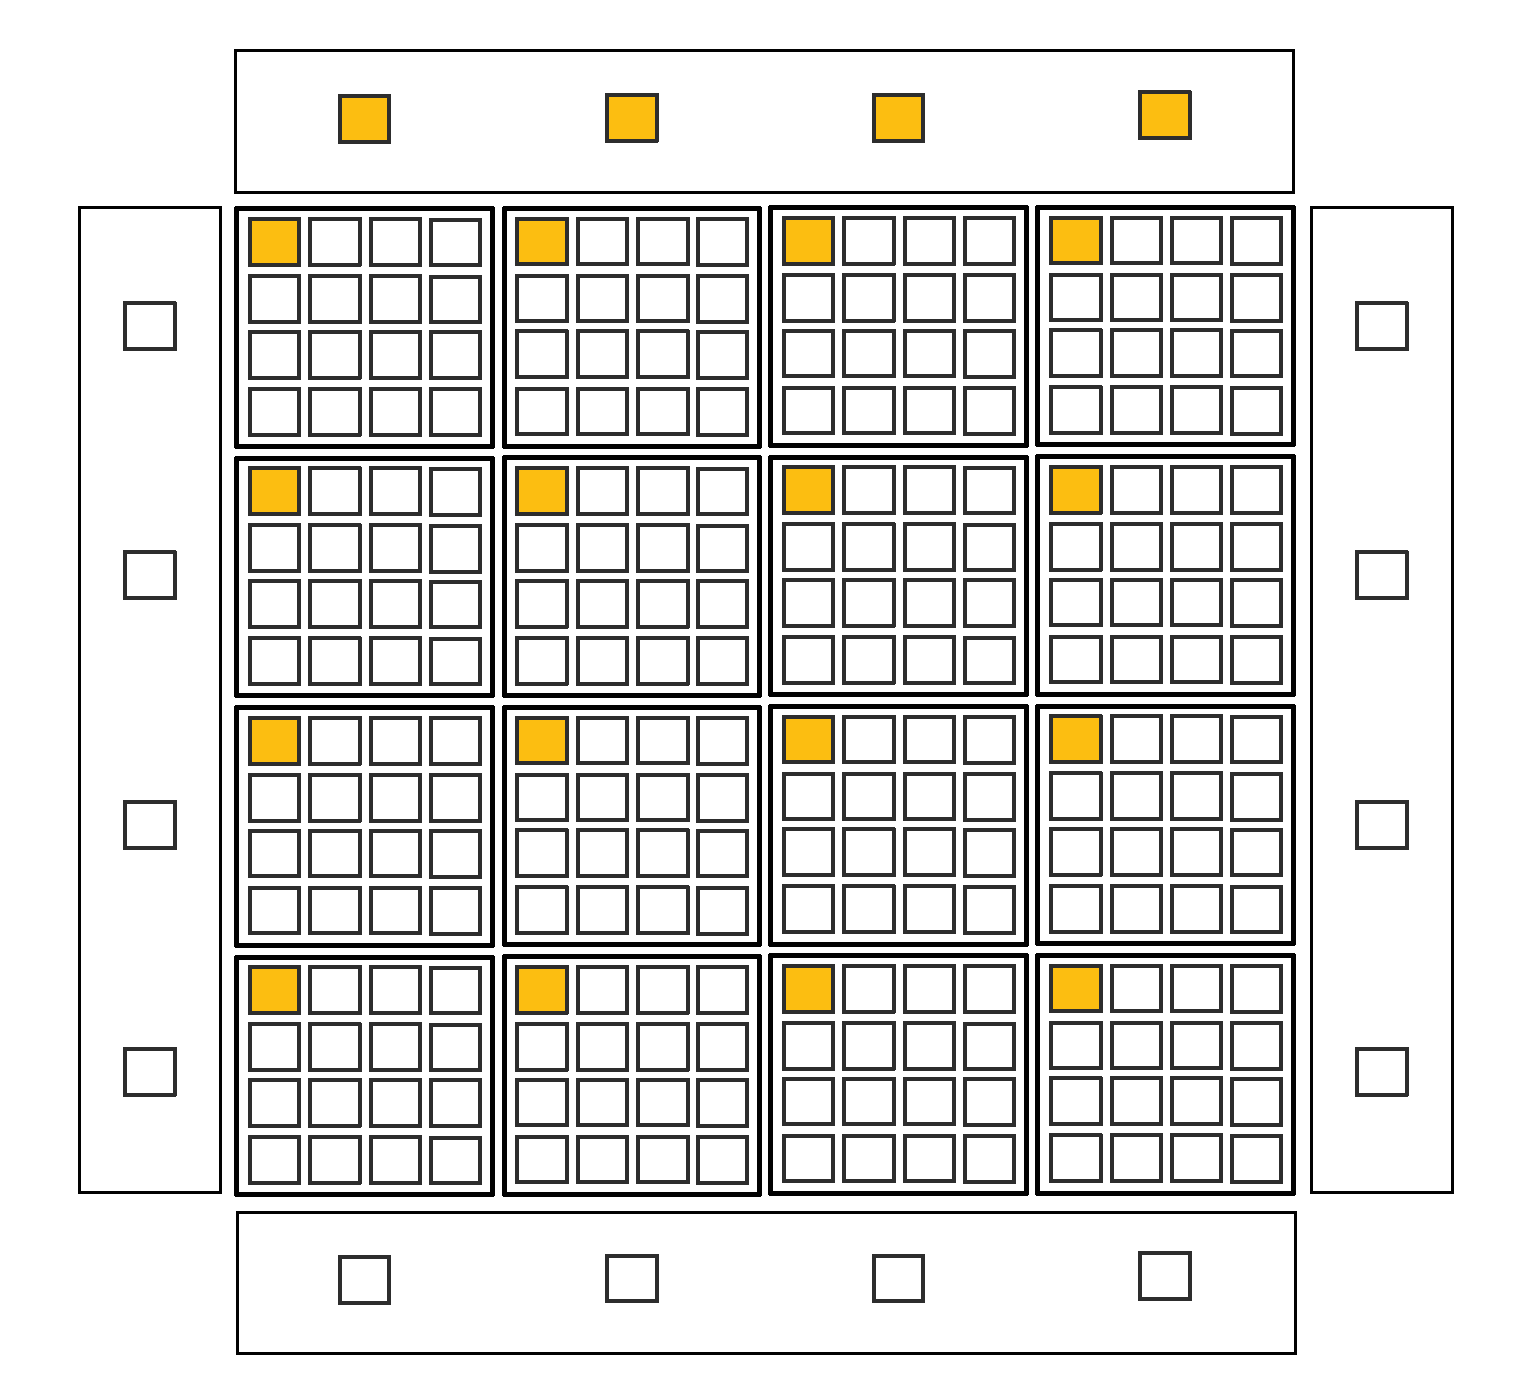
\includegraphics[width=1.0\linewidth]{../figure/ndt_matching.eps}
      \caption{\label{fig:ndt_matching_situation}
      A situation of vehicle self-localization execution.}
    \end{minipage}   
    &
    % \setcounter{figure*}{11}
    \begin{minipage}[!htbp]{0.49\textwidth}
      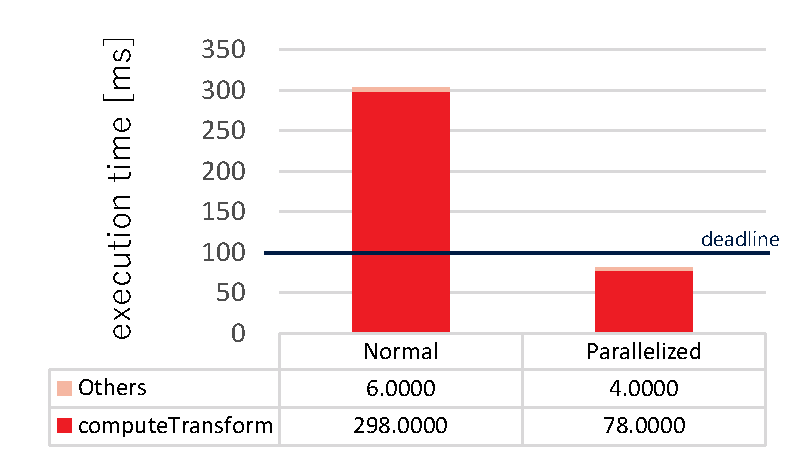
\includegraphics[width=1.0\linewidth]{../figure/BarGraph_ndt_matching.eps}
      \caption{\label{fig:ndt_matching}
      Vehicle self-localization of the partially parallelized self-driving application.}
    \end{minipage}
  \end{tabular}
\end{figure*}


\section{Lessons Learned}
\label{sec:lessons}
\comment{TBD: 3-4}
Thus far, in Chapter \ref{chap:evaluations}, we have quantitatively clarified the characteristic of data transfer and parallel computing on NoC-based embedded many-core platforms.
We can obtain insight and guidelines for users and developers of NoC-based embedded many-core platforms through MPPA-256.

From evaluations of D-NoC data transfer, we can learn two lessons: the influences of NoC routing and DMA.
First, data transfer latencies between clusters are hardly influenced by routing for users as shown in Figs. \ref{fig:DDR_tx}, \ref{fig:DDR_uc}, \ref{fig:IO_SMEM_tx}, and \ref{fig:IO_SMEM_uc}.
Software transactions of transmitting and receiving in routers and RM are dominant factors for latencies.
This is understandable owing to the minimized traffic conflicts of the evaluation setting.
However, when the influence of routing comes to intensive concurrent traffic over a large portion of the network, different routes might still have nontrivial impacts on the end-to-end data transfer delay, especially for a detour route of a longer length.
Second, in the IOS, the latency of a UC is not significantly affected by the memory location, the DDR or SMEM, at which the transferred buffer is allocated from the evaluation of Fig. \ref{fig:tx_uc_log}.
The merit of the UC is profitable for users because this is a common situation for transferring data from the DDR to the CC SMEM using the UC, especially for large amount of data.

From microbenchmarks of matrix calculation, we can learn three lessons of memory access: characteristics of the SMEM, influences of a cache, and data flow control on D-NoC.
First, the memory access speed of the CC SMEM exceeds that of the IO SMEM as shown in Fig. \ref{fig:mat_calc_uncache}.
There is a significant difference, which is a major reason to work actively in the CC.
Second, we indicate quantitatively that the calculation speed without the cache in the CC SMEM in Fig. \ref{fig:mat_calc_uncache} exceeds that with the cache in Fig. \ref{fig:mat_calc_cache}.
It is generally known that there is cache overhead when a miss hit occurs frequently, but it is notable that there is a substantial difference that cannot be ignored by the influences of a cache line.
Third, when data are transferred in parallel from multiple CCs to the IO DDR, NoC routers' FIFO sometimes overflows owing to memory access delays of the DDR.
This would ideally be expected to be prevented by the transmission protocol and flow control.

From the practical application viewpoint, since we parallelize the vehicle self-localization algorithm of the self-driving system, NoC-based embedded many-core systems can be used practically in real environments.
We applied for parallel data transfer from an IOS to CCs and parallel computing on the IOS and CCs by using the CC SMEM as scratch pad memory.    
We also conducted demonstration experiments with real environments and confirmed the practicality of NoC-based embedded many-core systems.

\chapter{Related Work}
\label{chap:related_work}
\memo{Add comparison to eMCOS, Facrored OS, and Barrelfish}
\memo{Add ROS-lite comparison table and descriptions}
This section compares many-core platforms and discusses previous work related to multi-/many-core platforms.
First, comparison of many-core platforms to other platforms is discussed.
Second, the Kalray MPPA-256 which this work focuses on is compared to other COTS multi-/many-core components, and we summarize the features of MPPA-256.
Finally, discussions of previous work and comparisons with them are described.

% Recently, studies indicate that the single core processors are characterized by limited computation performance.
% Pollack stated that a single core is inefficient \cite{pollack1999new} and that Moore's law \cite{moore2006cramming} is no longer applicable.
% Therefore, extant CPUs are not sufficient to satisfy increasing computation demands.
% The shift from a single core in real-Time and embedded systems has occurred \cite{saidi2015shift}. 
% Many other platforms including many-core are developed and researched by current studies.

Table \ref{tb:comparison_platforms} summarizes the features of many-core platforms with those of other platforms.
For instance, the GPU is a powerful device to enhance computing performance and has great potential in specific areas (for e.g., image processing, and learning).
\comment{1-24}
However, the GPU is mainly used for a specific purpose and its predictability is not suitable for real-time systems.
It is difficult to use a GPU for many kinds of applications and to guarantee its reliability due to the GPU architecture.
Many-core processors based on CPU are significantly superior to GPU with respect to software programmability and timing predictability.
\comment{1-25}
Additionally, it is commonly known that many-core platforms such as MPPA-256 involve a reasonable power consumption \cite{kanter2015kalray}.
In contrast, the GPU consumes a significant amount of power and generates considerable heat.
This is a critical problem for embedded systems.
FPGAs are also high-performance devices when compared to CPUs.
They are efficient in terms of power consumption.
FPGAs guarantee predictability and efficient processing.
% They are suitable for time-critical computing \cite{de2015kalray}.
\comment{1-26}
% However, DSPs cannot be used for many kinds of applications and programming.
However, FPGAs are difficult for software developers and are not a substitute for CPU since their software model is significantly different from that of CPU.
Many-core platforms can potentially replace single/multi core CPU as they possess ease of programming and scalability.

Based on the aforementioned background, many COTS multi-/many-core components are developed and released by several vendors.
(e.g., MPPA-256 by Kalray, \cite{de2014time}, Tile-Gx by Tilera \cite{ramey2011tile}, \cite{schooler2010tile}, Tile64 by Tilera \cite{bell2008tile64}, and Xeon Phi by Intel \cite{chrysos2014intel}, \cite{chrysos2012intel}, Single-chip Cloud Computer (SCC) by Intel \cite{baron2010single}).
The present work focuses on the Kalray MPPA-256, which is designed for embedded applications.
Kalray \cite{de2014time} presented clustered many-core architectures on the NoC that pack 256 general-purpose cores with high energy efficiency.


\comment{1-27}
MPPA-256 is superior to other COTS multi-/many-core components in terms of the scalability of the number of cores and the power efficiency, as shown in Table \ref{tb:comparison_manycore}.
\comment{1-28}
In terms of scalability, MPPA-256 uses 256 cores, whereas other COTS multi-/many-core components have 64 cores or the number of cores around it.
This scalability of cores is attributed to the NUMA memory architecture; each cluster of 16 cores contains its own local shared memory.
The precise hardware model is described in Section \ref{sec:hardware_model}.
When all cores share the global DDR memory as in other platforms excluding MPPA-256, specific bus/network routes receive extremely large loads and memory access contention frequently occurs.
Local shared memory reduces the above problems and helps the scalability of the number of cores.
% This is why MPPA-256 has succeeded in scaling up to 256 cores and what the ``scalability'' column of Table \ref{tb:comparison_manycore} means.
However, the NUMA memory architecture restricts the capacity of the memory and requires a data copy from the DDR with NoC.
This restriction makes the use of existing applications difficult especially in the case of applications that require more memory.
As a result, owing to the NUMA memory architecture, the portability of code porting to MPPA-256 is inferior to that of other COTS platforms, as shown in Table \ref{tb:comparison_manycore}.

In terms of power efficiency, MPPA-256 realizes superior energy efficiency despite its large number of cores \cite{kanter2015kalray}.
The total clock frequency per watt is the highest of the current COTS multi-/many-core components.
The power consumption of the MPPA processor ranges between 16 W at 600 MHz and 24 W at 800 MHz.
% While MPPA-256 and TILE64 \cite{bell2008tile64} target the embedded systems, other COTS components consider the HPC accelerator.
% Their clock frequency per core exceeds that of embedded solutions.
We must distinguish the COTS multi-/many-core components according to their requirements with reference to Table \ref{tb:comparison_manycore}.
MPPA-256 is typically accepted with respect to many-core platforms and the model has been used in previous work \cite{becker2016contention}, \cite{carle2014static}, \cite{perret2016mapping}, \cite{perret2016predictable}.

Previous work has examined real-time applications on many-core platforms, including MPPA-256.
Multiple opportunities and challenges of multi-/many-core platforms are discussed in \cite{saidi2015shift}.
The shift to multi-/many-core platforms in real-time and embedded systems is also described. 

Based on the above background, several task mapping algorithms for multi/many-core systems have been proposed \cite{carle2014static}, \cite{faragardi2014communication}, \cite{perret2016mapping}.
Airbus \cite{perret2016mapping} proposes a method of directed acyclic graph (DAG) scheduling for hard real-time applications using MPPA-256.
In \cite{faragardi2014communication}, a mapping framework is proposed on the basis of AUTOSAR which is applied as a standard architecture to develop automotive embedded software systems \cite{furst2009autosar}.
AUTOSAR task scheduling considering contention in shared resources is presented in \cite{becker2016contention}.

By examining the above mapping algorithms of real-time applications, previous work \cite{deDinechin2014GSN}, \cite{denet2017work}, \cite{kanter2015kalray}, \cite{perret2016predictable} has analyzed the potential of MPPA-256 and data transfer with NoC, as shown in Table \ref{tb:comparison_relatedwork}.
MPPA-256 is introduced and its performance and energy consumption are reported in \cite{kanter2015kalray}.
However, this report contains few evaluations and does not refer to data transfer with NoC and memory access characteristics.
Data transfer with NoC in MPPA-256 is described, and NoC guaranteed services are analyzed in \cite{deDinechin2014GSN} and \cite{denet2017work}.
While the theoretical analysis is thorough in these works, the practical evaluations are poor and parallel data transfer is not referred to.
The authors of Ref. \cite{perret2016predictable} focused on the predictable composition of memory access.
An analysis of their work identified the external DDR and the NoC as the principal bottlenecks for both the average performance and the predictability on platforms such as MPPA-256.
Although the analysis examined the memory access characteristics of the external DDR and provided notable lessons, a solution for the DDR bottleneck was not examined and practical evaluations were lacking.

\begin{landscape}
  % \renewcommand{\arraystretch}{1.2}
  \begin{table*}[!htbp]
    \caption{\label{tb:comparison_platforms}
      Comparison of Many-core Platform to CPU, GPU, and FPGA}
    \centering
    % \scriptsize	                    % text size
    % \tabcolsep = 0.4mm              % side-margin in column
    \begin{tabular}{c|cccccccccc}
      \hline
      & \multirow{2}{*}{performance} & \multirow{2}{*}{power/heat} & \multirow{2}{*}{real-time} & software & \multirow{2}{*}{costs} & multiple\\
      &&&&& development & instruction \\
      \hline
      \hline
      CPU & & L & \(\checkmark\) & \(\checkmark\) & \(\checkmark\) & L \\
      GPU & \(\checkmark\) &  &  & L & \(\checkmark\)\\
      % DSP & L & L & \(\checkmark\) & \(\checkmark\) & L & \(\checkmark\) & \\
      FPGA & \(\checkmark\) & L & L &  & L & \\
      Many-core Platform & \(\checkmark\) & \(\checkmark\) & \(\checkmark\) & \(\checkmark\) & L & \(\checkmark\) \\
      \hline
    \end{tabular}
    \begin{flushright}
        \comment{1-23} \textasteriskcentered In a table, ``L'' means ``limited''.
    \end{flushright}
  \end{table*}

  % \renewcommand{\arraystretch}{1.2}
  \begin{table*}[!htbp]
    \caption{\label{tb:comparison_manycore}
      Comparison of Many-core Platforms}
    \centering
    % \scriptsize	                    % text size
    % \tabcolsep = 1.5mm              % side-margin in column
    \begin{tabular}{c|cccc}
      \hline
      & \multirow{2}{*}{scalability} & power  & code & \\
      & & efficiency & transplant & \\
      \hline
      \hline
      Kalray MPPA-256 \cite{de2014time} & \(\checkmark\) & \(\checkmark\) & L & \\
      Tilera Tile series \cite{bell2008tile64} &  & L & \(\checkmark\) & \\
      Intel Xeon Phi \cite{chrysos2014intel} \cite{chrysos2012intel} &  &  & \(\checkmark\) & \\
      Intel SCC \cite{baron2010single} &  &  & \(\checkmark\) & \\
      \hline
    \end{tabular}
  \end{table*}  
  % \renewcommand{\arraystretch}{1.2}
  \begin{table*}[!htbp]
    \caption{\label{tb:comparison_relatedwork}
      Comparison of Previous Work}
    \centering
    \scriptsize	                    % text size
    % \tabcolsep = 2mm              % side-margin in column
    \begin{tabular}{c|ccccccccc}
      \hline
      & performance & data transfer & memory access & \multirow{2}{*}{real applications} & parallel data & \\
      & analysis & analysis with NoC & characteristics & & transfer & \\
      \hline
      \hline
      Kalray clusters calculate quickly \cite{kanter2015kalray} & L &  &  &  &  & \\
      Network-on-Chip Service Guarantees \cite{denet2017work} &  & \(\checkmark\) &  &  &  & \\
      Predictable composition of memory accesses \cite{perret2016predictable} &  & \(\checkmark\) & \(\checkmark\) &  &  & \\
      this paper & \(\checkmark\) & \(\checkmark\) & \(\checkmark\) & \(\checkmark\) & \(\checkmark\) & \\
      \hline
    \end{tabular}
  \end{table*}
\end{landscape}


\chapter{Conclusions}
\label{chap:conclusion}
% This paper has conducted quantitative evaluations that examined end-to-end latencies with embedded many-cores based on NoC, the scalability of parallelization, and the characteristics of the memory access speed.
% From various experiments, we have evaluated the capabilities of the currently available data transfer methods and the parallelization potential for many-core computing based on NoC.
% Our experimental results will allow system designers to choose appropriate system designs based on the requirements of their latency-sensitive many-core applications beyond an intuitive expectation.
In this work, we conducted quantitative evaluations of data transfer methods on NoC technology, microbenchmarks with matrix calculation, and a practical application with NUMA many-core platforms such as MPPA-256.
Evaluations indicate latency characteristics on NoC platforms, influences of data allocation, and the scalability of parallelization.
Our experimental results will allow system designers to select appropriate system designs.
Last, parallelization of a real application proved the practicality of NoC-based embedded NUMA many-core platforms.

In future work, we will use benchmark applications such as that in \cite{che2010characterization} for further analysis.
In addition, considering above the results, we will port real-time systems such as that in \cite{maruyama2016ros2} on CCs, and we propose the parallelization of memory intensive algorithms, such as the nearest neighbor search in Section \ref{sec:practical_application}.


%%%%%%%%%%%%%%%%%%%%%%%%%%%%%%%%%%%%%%%%%%%%%%%  テンプレート非依存部(終了)  %%%%%%%%%%%%%%%%%%%%%%%%%%%%%%%%%%%%%%%%%%%%%%%  


% use section* for acknowledgment
% \ifCLASSOPTIONcompsoc
  % The Computer Society usually uses the plural form
  % \chapter*{Acknowledgments}
% \else
  % regular IEEE prefers the singular form
%   \chapter*{Acknowledgment}
% % \fi
%   This paper was partly supported by Toyota Motor Company, eSOL, and Kalray.
%   In addition, this research was partially supported by JST, PRESTO.

% \ifCLASSOPTIONcaptionsoff
  % \newpage
% \fi

% \renewcommand{\baselinestretch}{0.8}

% \comment{2-5}
% \comment{TBD: 3-6}
% \bibliographystyle{IEEEtran}
% \bibliography{./reference.bib}

% \end{document}

